\documentclass[MScCS]{uccthesis}
\usepackage{graphicx,wrapfig,lipsum}
\usepackage{float}
\usepackage{subcaption}

\title{Mobile Application For Visually Impaired Individuals}
\author{SHUBHAM KAREKAR}
\supervisor{DR. SABIN TABIRCA}
\secondreader{DR. JOHN HERBERT}
\date{\today}

\newcommand*{\COMMAND}[1]{\texttt{\textbackslash #1}}
\newcommand*{\COMMANDWITHARGUMENT}[2]{\texttt{\textbackslash #1}\{#2\}}

\addbibresource{mybib.bib}% should be in preamble

\abstract{%
   This thesis presents the initiative to create a android smartphone application for visually impaired people that will give audio feedback, object identification, and distance measurement features to help them in their day to day life. To give accurate and dependable findings, the program will employ image processing techniques, machine learning technologies such as ML-Kit and Tensor Flow, artificial intelligence approaches as well as implementing computer vision techniques. The idea was inspired by the desire to boost the standard of living and mobility of visually impaired people, who frequently struggle with item recognition, text reading, and recognizing people. The development of an easy-to-use interface, accurate object identification, and distance measurement are the main hurdles in the application's development. The application will be evaluated based on important performance indicators such as accuracy, precision, and recall.\\
   \\The application will provide a simple interface which will be easy to use for the visually impaired individuals so they can seamlessly navigate via intuitive gestures. This dissertation demonstrates a dedication to transparency and diversity. subsequently not only displays an advantageous use but also emphasizes the significance of easily available innovation for solving practical problems.


   
}

%\dedication{%
%   Your dedication here.
%}

%\acknowledgement{%
%   Your acknowledgement here.
%}

\renewcommand\addToFrontMatter[0]{%
}

\begin{document}
   \chapter{Introduction}
   In the report's Introduction chapter, we explore the crucial problem of blindness, which impacts more than two billion individuals globally and poses serious problems for their autonomy and happiness. In order to help people with visual impairments, we highlight the necessity for user-friendly navigational aids and accessible technologies in cities. Our novel application's goals and aims are outlined. It uses artificial intelligence and machine learning methods to deliver real-time aural feedback regarding words, persons, and things. The revolutionary results obtained via the integration of this ground-breaking technology, boosting connectedness and providing assistance for those with visual impairments, are highlighted in the end of the chapter.

   \section{General Facts}
  Data show that many of individuals globally suffer from a form of blindness, which is defined by various degrees of vision loss, and that it is highly prevalent across a wide range of groups. This condition seriously interferes with daily activities and threatens independence and overall health. Visually challenged people must navigate the complexities of this battle and face challenges with communication, education, work, and integration into society. \\
   \\
   There are over 2.2 billion visually handicapped people around the world. When navigating their environment, these people face a number of problems.\\
    \\
    Blind people can wander easily throughout their home since they are familiar with the layout of each area. But once they leave their homes, they could run across problems. Visually impaired people frequently experience difficulties with object identification, text reading, and recognising familiar faces, which can result in a decline in independence and an increase in dependency on others. They are unable to lead satisfying lives as a result, which has an impact on both their everyday activities and possibilities.
   \section{Particular Facts}
    The absence of readily available and intuitive navigation aids for those with visual impairments in urban environment is the main issue addressed by this study. The requirement for flawless screen reader integration, touch-based connections, and interoperability with a variety of assistive devices leads to technical limits. Given the availability of solutions, visually impaired people frequently encounter difficulties with effectively navigating their surroundings, carrying out tasks, and getting access to crucial information. For instance, misunderstanding and irritation are sometimes caused by the erroneous audio signals provided by present programs. These limitations have an impact on the design of our program, which attempts to deliver precise real-time navigation guidance while taking into account the particular difficulties faced by visually impaired users. Substantial psychological impacts result from difficult navigational experiences, including emotions of dependence on others, loneliness, and low self-esteem. Visually Impaired Individuals face many challenges which can cause a lot of trouble for them. Making their life easier via technology.
    
   \section{Aim and Objectives}
   \subsection{Aim}
   The aim of this project is to create an Application that enables blind and visually impaired people to independently and with greater confidence explore their environment. To deliver auditory feedback on words, people, and objects in the surroundings, the app will make use of computer vision, machine learning.\\
   \\Slider motions are going to be used to construct this program, which will have a significant influence on people. Finally, the dissertation seeks to contribute to the greater drive to advance equality and accessibility for those with impairments, particularly in the area of innovation.


   \subsection{Objectives}
   The following are the objectives of the application:-
   \begin{itemize}
       \item Developing a Robust Application which can detect object, people and text in a real time scenarios.
       \item Designing a user-friendly text-detection interface that will capture all the text in the vision of the user and provide a auditory feedback of the words recognized. 
       \item Building an environment-specific object recognition screen that enables individuals to recognize and engage with diverse objects. Using innovative object identification algorithms to precisely classify and define items that are observed.
       \item Delivering an intuitive design which allows individuals to quickly and easily slide among the activities. Ensuring that audio cues assist users when they switch between the activities.
       \item Measuring the distance between the user and the identified objects or the people, integrating distance measurement capability into the app's interface. 
       \item Implementing an auditory output system that speaks the outcomes of text, object, and people detection as well as estimating the distances in a straightforward and lucid manner. 

   \end{itemize}

   \section{Outcome}
   The integration of this intriguing application has resulted in a breakthrough approach that dramatically improves connectivity and backing up the visually impaired people. The application enables users to engage with and comprehend their environment with greater effectiveness by seamlessly incorporating text, people, and object identification features with audio feedback and measurement of distance.\\
   \\The following objectives has been achieved:-
   \begin{itemize}
       \item Real-Time text, object and person detection with the help of a android camera.
       \item All the detection is achieved by a video interface.
       \item Text-Detection functionality can efficiently capture all the text coming in the vision of the user.
       \item Auditory feedback has been implemented so that the users can get the information through a voice for all the things coming in there way.
       \item User friendly interface has been implemented. The audio cue announces the name of the screen each time user switching the screen with slide gesture.
       \item Another distinctive characteristic of the application is the ability to calculate and offer measurements for the distance between identified items or person and the user. 
       \item Object Recognition Functionality can identify wide range of objects including chairs, tables, laptop, people \textit{etc.}
   \end{itemize}
\newpage


   \section{Outline of the Report}

   This section describes the outline or the structure of the report.

   \begin{enumerate}
       \item \textbf{Chapter 1 - Introduction }\\
       The Introduction chapter briefly describes the facts and and the problems faced by visually impaired individuals. Also provides the aim and the objectives of the application. The chapter eventually briefs about the outcome of the app.
       \item \textbf{Chapter 2 - Literature Review and Background}\\
       This chapter presents all the related work in form of Research papers and similar application, providing insights about them. It also consist of the Background section which describes the technologies and the computer vision techniques used in the application.
       \item \textbf{Chapter 3 - Analysis}\\
       The various tasks performed by the by the application are briefly described in this chapter.Functional and non-functional requirements are detailed throughout this chapter.
       \item \textbf{Chapter 4 - Design}\\
       This Chapter consider overall design of the developed application and states various use cases. It also provides information about the back-end of the application.
       \item \textbf{Chapter 5 - Implementation}\\
       Technical implementation and proposed application's functionality has been described in this chapter. This chapter gives an in-depth look at the technical principles that allow those with disabilities to interact with an engaging and instructive application interface, leading to their greater access and interaction with their surroundings.
       \item \textbf{Chapter 6 - Testing}\\
       "Testing" chapter provides an in-depth review of the application's efficiency, accessibility, and overall user experience. It has systematically examined the precision of text, persons, and object detection capabilities, measuring their success and failure rates, using a set of supervised tests for usability.
       \item \textbf{Chapter 7 - Conclusion}\\
       The Conclusion Chapter has presented how the application dealt with numerous issues and how it has been solved.
   \end{enumerate}

   
\chapter{Literature Review And Background}
This chapter defines the problems, solution, techniques, relevant work and tools that will be used to build a Mobile Application for Visually Impaired Individuals. This chapter gives an overview of existing information and expertise about the subject topic.The purpose of this chapter is to show that the study is guided by relevant and current information, and that the suggested strategy is realistic and promising.
\section{Literature Review}
\subsection{Literature Review Methodology}
The technique used in this study for the literature review systematically directed the choice and evaluation of pertinent academic articles. To begin, particular inquiries were developed to give an organized structure to the analysis. Following that, an extensive search approach was developed, which included significant academic search engines, journals with peer review, and trustworthy web sources relevant to the subject of the study topic.\\
\\
The search was boosted with the help of search engines such as \textit{"Google Scholar"} and various sites like \textit{"UCC CORA"}. The search has been conducted using multiple keywords like "Machine Learning", "Object Recognition", "Text Recognition",\textit{etc.}Following the first search, a continuous filtering procedure was carried out, comprising an in-depth evaluation of books, descriptions, and entire contents to discover articles that matched with the study's aims.  The accuracy and legitimacy of the original sources were ensured by evaluating the quality of the material that was chosen. While the technique attempted to assure thoroughness and precision, multiple drawbacks, such as dialect obstacles and connectivity constraints, were discovered. 

\subsection{Related Work}
\subsection{Research Papers}
\begin{enumerate}
        %\item   \textbf {Assistive Mobile Application for Visually Impaired People}
        \item \textbf{\Parencite{Assistive}}-  The project discussed in the article is an assistive mobile application for visually impaired persons. The app's goal is to make persons with visual impairments' life easier by offering them with a variety of beneficial features and capabilities.Voice recognition, text-to-speech conversion, and obstacle detection are among the functions included in the program. The voice recognition capability allows users to speak instructions and the app will answer, whilst the text-to-speech option reads text from the device's screen. The obstacle detection function detects obstructions in front of the user and provides an audible alert to warn them.

Devices Used:-\\
1. Android Phone as a primary device


%\item  \textbf{Object recognition in a mobile phone application for visually impaired users. }
\item \textbf{\Parencite{Obj}}-  The goal of the study, as detailed in the paper, is to create a mobile phone application that can recognise objects for users who are blind or visually impaired. The program takes pictures of items with a mobile phone camera and then uses image-processing techniques to recognize the objects in the pictures. The user is then given an audio description of the object by the program.

The Android platform was used to create the program, and the developers tested it on the Sony Xperia S and Samsung Galaxy S II smartphones. For image processing and word recognition, the authors also employed the Tesseract OCR engine and the OpenCV library. The initiative intends to increase the freedom of visually impaired people and enhance their quality of life.

Devices Used:-\\
1. SmartPhone Camera


%\item \textbf{Distance Assessment by Object Detection For Visually Impaired Assistive Mechatronic System }
\item \textbf{\Parencite{distance}}- The paper demonstrates a method that employs object detection to determine distance in a visually impaired assistive mechatronic system.

A camera and a microcontroller board with image processing capabilities are included in the system. The camera takes pictures of the environment, which are subsequently analysed by the microcontroller using a deep learning-based object identification algorithm. Based on their sizes and locations in the image, the algorithm recognises items in the scene and determines their distances.

The system provides the individual with real-time feedback in the form of auditory cues that indicate the distances between the detected objects.

Devices Used:-\\
1. Camera \\
2. Microcontroller





%\item \textbf{Real-time object detection and face recognition system to assist the visually impaired} 
\item \textbf{\Parencite{RTOD}}-  The research describes a real-time recognition of the objects and face detection system aimed at assisting those with visual impairments. For object detection, the system employs a deep learning-based technique, especially the Single Shot Detector (SSD) algorithm. The system recognises faces using a pre-trained deep neural network.

When an item or a face is identified, the system produces an audio output to notify the user of the object's existence or the identification of the recognised face. A text-to-speech (TTS) engine turns the text into voice to provide the audio output.

The system was built and tested using a Raspberry Pi 3B+ board and a Raspberry Pi camera. The authors reported object detection accuracy of 92.3% and face recognition accuracy of 96.4%.

Devices Used:-\\
1. Camera\\
2. Raspberry Pi board



%\item \textbf{Smart Glass System Using Deep Learning for the Blind and Visually Impaired} 
\item \textbf{\Parencite{smartglass}}- To identify and recognise objects and text in the user's environment, the system use a combination of deep learning algorithms and computer vision techniques. The system is intended to be worn, with the smart glass display put directly in front of the user's eyes.

The smart glass system captures photos of the user's surroundings via a camera, and the images are then processed with deep learning algorithms to detect and recognise objects and text. A text-to-speech capability is also included in the system, which reads aloud the detected text to the user.

Devices Used:-\\
1. Camera\\
2. Display\\
3. Micro-controller\\
4. Speaker\\


%\item \textbf{Collaborative Music Application for Visually Impaired People with Tangible Objects on Table}
\item \textbf{\Parencite{collaborative}}- It provides a collaborative music application developed to ease music composition for visually challenged persons. The authors use tangible objects on a table as the application's input method.

The setup comprises of a table with a camera and a projector put on top. The camera detects the position and orientation of the tangible objects, and the projector displays visual feedback on the table surface. The actual items utilised are little wooden blocks, each of which symbolises a musical note or instrument.

The application provides a user interface that allows users to create music by placing and moving the tangible objects on the table.

Devices Used:-\\
1. Table\\
2. Camera\\
3. Projector\\
4. Tangible Objects: Small wooden blocks that represent musical notes or instruments. These objects are used as the input method for the music creation process.

%\item \textbf{CICERONE- A Real Time Object Detection for Visually Impaired People}
\item \textbf{\Parencite{cicerone}}- The article explains the CICERONE technology, which is a real-time object detection system developed to help visually impaired persons.
The technology analyses the video feed and identifies items in the user's environment using machine learning techniques.

The CICERONE system is meant to function in real-time, which means that object detection and recognition happens in milliseconds. Its quick processing time allows visually impaired individuals to obtain instant input about their surroundings, making it easier and safer for them to manage their environment.

To evaluate the video feed and identify objects, the system employs deep learning methods, notably convolutional neural networks (CNNs).

Devices Used:-\\
1. Android Phone


%\item \textbf{Sensor-Based Prototype of a Smart Assistant for Visually Impaired People Preliminary Results}
\item \textbf{\Parencite{sensor} }- The goal of this project is to use sensor-based technologies to create a smart assistant prototype for those who are vision impaired. The intelligent assistant is intended to recognize obstructions and provide users instructions through audio feedback.

The speaker and servo motor are used to give the user directional feedback, and the camera module and ultrasonic distance sensor are utilized to identify obstacles. The primary processing unit for the system is the Raspberry Pi computer, which also manages how the other gadgets work.The navigation is served offline to the users

Devices Used:-\\
1. Raspberry Pi 4 Model B computer\\
2. Servo Motor\\
3. Ultrasonic distance sensor\\

%\item \textbf{Interactive Sound Generation to Aid Visually Impaired People via Object Detection Using Touch Screen Sensor} 
\item \textbf{\Parencite{interactive}}- According to the article, the aim of this research is to make a program that can generate interactive sounds to aid impaired individuals in object recognition using a touch screen sensor.

A touch screen sensor is used by the system to identify the presence and position of an object put on it. When an item is recognized, the system produces an interactive sound that conveys information about the shape, texture, and other aspects of the object. The system may also emit distinct noises for various things, allowing the user to differentiate between them.

Overall, this experiment indicates the possibility of integrating touch screen sensors and interactive sounds to assist visually impaired persons with item detection, thereby increasing their independence and quality of life.

Devices Used:-\\
1. Touch Screen Sensor\\
2. Microcontroller (Arduino Uno)\\
3. Speaker\\
4. Power source

%\item \textbf{An Embedded Application for Degraded Text Recognition} 
\item \textbf{\Parencite{embedded}}- An embedded system for identifying degraded text is shown. The system is intended to detect text that has been degraded as a result of poor resolution, low contrast, and noise, which can occur in a variety of real-world settings such as mobile picture capture and document scanning.

The system's technology is based on a mix of image processing and pattern recognition algorithms. The system begins by preprocessing the input image in order to improve its quality and eliminate noise. The image is then processed using a feature extraction approach based on wavelet transformations. The collected characteristics are then used to train a classifier using the support vector machine (SVM) technique.

Devices Used:-\\
1. Texas Instruments OMAP5910 board: Is an embedded system-on-chip (SoC) that combines an ARM926EJ-S processor with a TMS320C55x DSP core. The board is used for implementing the image processing and pattern recognition algorithms in real-time.\\ 
2. Camera module

\end{enumerate}
\subsection{Applications}
\begin{enumerate}
    \item \textbf{Be My Eyes - IOS Application - https://www.bemyeyes.com/}

Working:-
Be My Eyes application lets a user to connect with a sighted volunteer around the world, who     will help them to describe the objects, faces etc through a video call. 
The app requires the user to sign up in the application before starting.
It has to options to either be a volunteer for a visually impaired  individual or be the user of the application by calling the volunteer
The volunteer will receive a notification once the user will tend to call a volunteer.
The user can end the call when the task is over.

Cons:-
The volunteer might not be available for the immediate help needed to the user.
Volunteer can see everything that the user will show to him/her, which can raise privacy concerns.
\\
\\\item \textbf{Seeing AI - IOS Application - https://www.microsoft.com/en-us/ai/seeing-ai}

Working:-
Seeing AI is an application developed by Microsoft.
The software can detect a broad variety of items and scenarios, including people, text, goods, colours, and more. For example, a user may aim their phone at a can of soup, and the software will detect the label and read it aloud. 
Alternatively, a user may hold their cell phone up to a sign and the software will read the words on the sign.

Cons:-
Only available on IOS
Initial users may find it difficult to operate.

\item \textbf{TapTapSee - IOS Application - https://taptapseeapp.com/}

Working:-
The application captures the image and uses image recognition technology to identify the objects in the image.
The task of the user is to simply point the camera towards the environment and double-tap to capture the image.
After the image has been captured, the application identifies the objects and provides the audio description of it.

Cons:-
Requires internet connection

\item \textbf{RightHear - IOS Application - https://www.right-hear.com/}

Working:-
The application is initially opened it requires permission to use mobile's bluetooth connection.
The application navigates the user's current location and outputs the location in an auditory format.
The application also provides information about the surrounding streets, stores, etc.
Whenever the user touches the screen the application scans the environment and describes it.

Cons:-
Provides inaccurate information if bluetooth beacons are not available in the locality.
The application provides only one functionality of navigating.

\item \textbf{EyeCYou - IOS Application - https://eyecyou.dk/}

Working:-
The application uses mobile's camera to capture image, the user only needs to touch the screen to capture the image.
The application then uses image recognition technique to identify whether there is a person or not.
If there is a person in the image, the application describes the person in a detailed manner.

Cons:-
The Application has only one functionality to describe a person.
It does not define a object which is more complex or unique.

\item\textbf{TalkBack - Android Accessibility Feature - support.google.com/accessibility/android}

Working:-
It is a accessibility feature which is in-built in many Android Phones.
Talkback uses gesture based navigation through the device so visually impaired users can easily navigate.
It provides auditory feedback to define the menu, app names, user interface etc.
Talkback announces the name of the item when it is selected.

Cons:-
Some applications are not compatible with this accessibility feature, which may make difficulties in accessing feature of that application

\item \textbf{SuperSense AI for Blind - Android Application - https://the.supersense.com/}

Working:-
App uses Artificial Intelligence to identify and recognise objects.
Supersense uses device camera to scan the objects in the vision
It provides auditory feedback describing the objects and elements which has been detected by the application .
It also has a Scene Description Feature which provides more detailed information.

Cons:-
Does not provide accurate information

\item \textbf{Lookout - Android Application - https://www.lookout.com/}

Working:-
Lookout is developed by Google.
The app has many modes which are identifying the objects in surrounding, scanning a document, quick read function which reads text from messages or email and currency mode which can be used to identify the currency.
The application provides audio feedback once the application has scanned the image and the objects in the image.

Cons:-
Limited functionality



\end{enumerate}


\subsection{Overall Insights}

Overall, these articles of research as well as applications illustrate important advances in the development of technology that helps to better improve the daily lives of those with visual impairments. The utilization of contemporary technology, such as cellphones, recording devices, and deep machine learning processes to produce new approaches is an ongoing theme throughout these research. \\
\\
In these papers and applications wide range of technology is used such as Rasberry pi, Microcontroller, Servo Motor, OMAP5910 board, Ultrasonic Sensor \textit{etc.} This range of devices exhibits the versatility of technology that adapts to different circumstances and choices.\\
\\
Methods based on deep learning, notably neural networks using convolution (CNNs), are crucial in a number of studies involving identifying objects and translation of text into speech. This highlights the significance of machine learning in improving the capacity of assistive devices. All these shows a good impact of these studies on technological world. These highlight the power of innovation to close barriers and improve equality and inclusion for everyone.

\subsection{Conclusion of Articles and Applications}
A unifying pattern appears in this set of studies and applications: a commitment to utilize innovation to better the lives of those with visual impairments. These papers/applications highlight a variety of new ideas, gadgets, and procedures aimed at improving the autonomy and standard of life of people with vision problems.\\
\\
In addition, some research highlight the significance of sound signals and participatory sounds in communicating data to individuals with visual impairments. Such aural input techniques, in conjunction with speech-to-text and text-to-speech engines, help consumers have a more engaging yet instructive interaction.

%\section{Problem Description}
%This initiative of my project addresses the issue of visually impaired people's loss of freedom and movement. When it comes to navigating their surroundings, blind and visually impaired persons confront a number of challenges, such as item recognition, text reading, and identifying familiar faces. There is a 45\% higher risk of having a road traffic crash.
%\begin{figure}[hbtp]
      %\hrule
     % \vspace{0.5em}
     % \centering
      %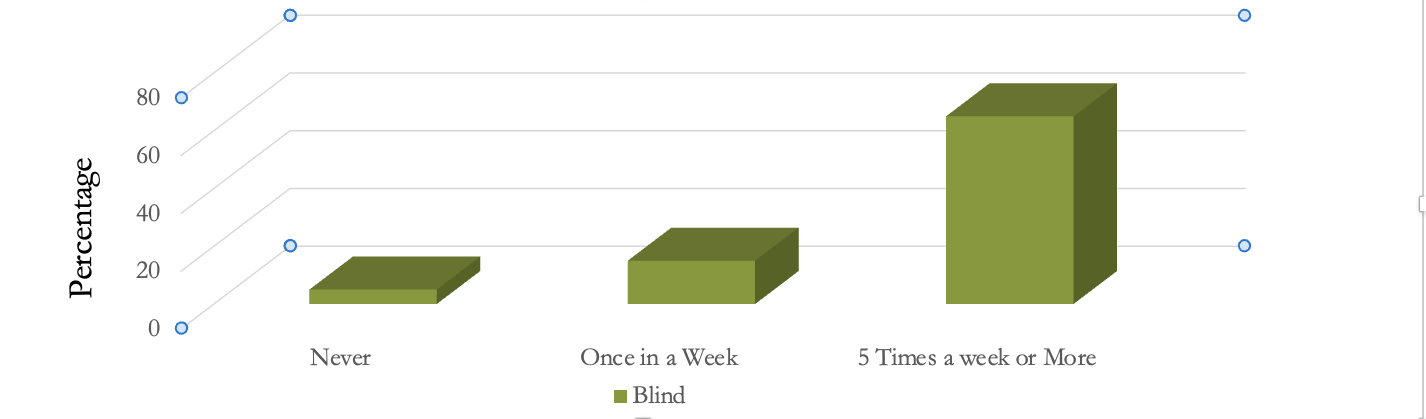
\includegraphics[width=0.95\textwidth]{Figures/Graph.png}
     % \vspace{0.5em}
     % \hrule
     % \caption{\label{fig:including@a@picture}No.of Accidents per week vs Percentage }
      %\vspace{0.5em}
      %\hrule
   %\end{figure}
%These difficulties can lead to a loss of independence and an increase in reliance on others. As a result, there is a need for an application that may help visually impaired people manage their daily lives more efficiently, allowing them to live more fulfilling lives with improved freedom and mobility.




%\section{Solution} 
%.For the problem that have been mentioned in this paper, the proposed application is a proper solution. The application will capture pictures of the surroundings using the smartphone camera, and machine learning algorithms will recognize messages, identifiable faces, and objects. The program will then employ text-to-speech technology to offer users with audio feedback, identifying the items and messages in the image and recognizing familiar faces. The process will be done using Smart Glasses or a small camera on the user for capturing the images and processing it to the application. Some of the features of the application are listed below:-
%\begin{enumerate}
    %\item Object Recognition - Using Computer Vision techniques and machine learning algorithms the app can determine the object by image processing. The image which has been transferred to the application by the hardware device is been processed to identify the object.
    %\item Face Recognition - The software may utilize the camera to capture a photograph of a person's face then utilize a pre-trained model to identify the person. When a person is detected, the app can send audio feedback alerting the user of the individual's name.
    %\item Distance Measuring - Using an Ultrasonic sensor the application can measure the distance between the individual and the object and provide it to the user in an auditory feedback.
    %\item Text Recognition - The software will employ optical character recognition (OCR) to recognize and read aloud the text in the surroundings, making it possible for those who are blind or visually impaired to read signs, store names, and other messages.
    %\item Auditory Feedback - Text-to-speech (TTS) technology is used by the program to turn identified objects, faces, and text into audible feedback for the user. To deliver more natural-sounding audio, TTS technology may be trained using a voice dataset.
%\end{enumerate}

%\subsection{Flow of Tasks}\begin{figure}[hbtp]\hrule\vspace{0.5em}\centering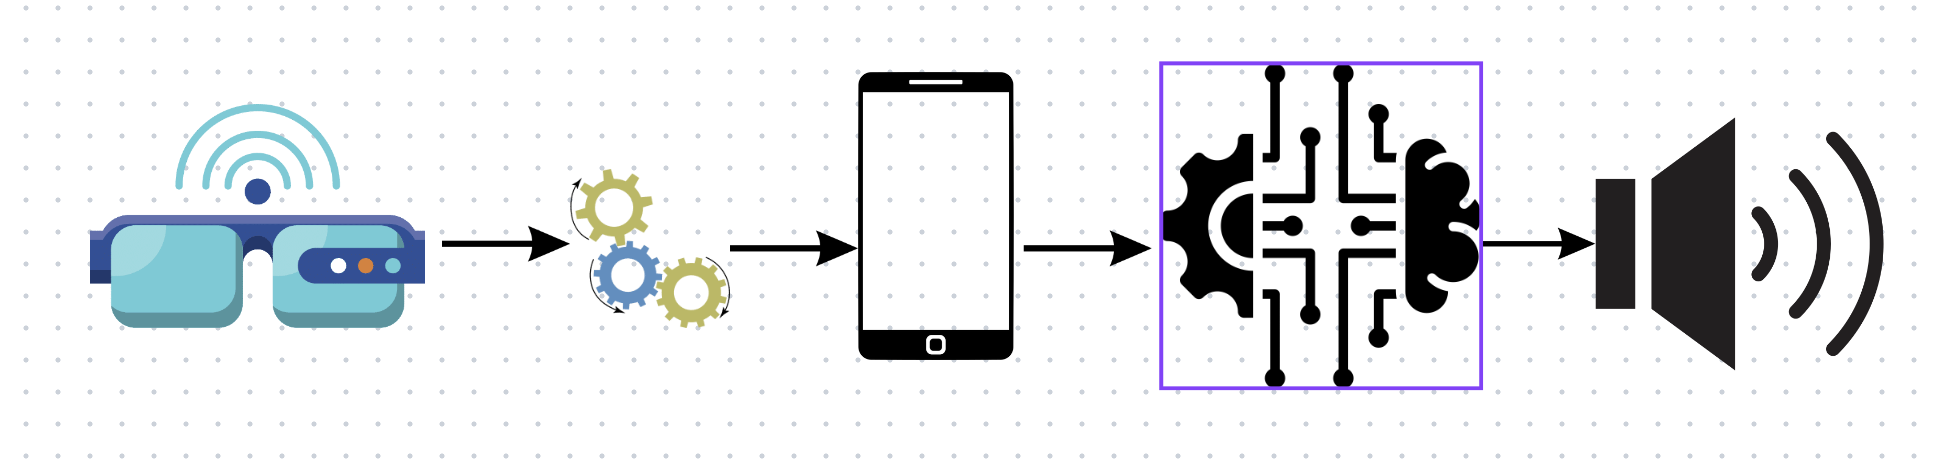
\includegraphics[width=0.95\textwidth]{Figures/flow.png}\vspace{0.5em}\hrule\caption{\label{fig:flow}Execution of Tasks }\vspace{0.5em}\hrule\end{figure}
%As shown in the figure \ref{fig:flow} the execution of tasks initially takes place by capturing the images from the smart glass or a small camera which will be transferred to the application that will be processed by the computer vision and machine learning techniques. The processed information will be transferred to the output speaker. Then the auditory feedback will be provided to the user via speaker.

\section{Personal Conclusion}
Examining the aforementioned publications reveals that the field of science is making a determined effort to create cutting-edge innovations that will enhance the standard of existence for those who are blind or visually impaired. These methods make use of different pieces of computer software and hardware to offer fundamental features including textual and object recognition, recognizing obstacles, and aural feedback.\\
\\These studies demonstrate the variety of feasible options by addressing the difficulties experienced by individuals with vision impairments in distinctive ways. Particularly, the creation of such supportive devices is greatly aided by the application of deep computing, machine learning, methods for computer vision, and sensor-based innovations.\\
\\The goal of these publications is to increase the autonomy, availability, and participation of people who are blind or visually impaired. In addition to providing workable answers for daily problems, these advances in technology also help to lessen emotions of reliance, loneliness, and lack of self-worth.\\
\\It is also heartening to see how mobile phones, digital cameras, micro-controllers, and various other easily accessible hardware parts are being combined to provide affordable and easy to use solutions. These initiatives support the overarching objective of increasing the accessibility of assistive technology to more people.\\
\\The study material discussed in these publications highlights the significance of constant advancement in aids for the blind. Thousands of people's lives might be considerably improved by such advances, which could close loopholes and provide their interests with greater autonomy and liberty as they travel over the globe.


\section{Background}
\subsection {Computer Vision, Machine Learning and\\ Artificial Intelligence}
In recent years, assistive technology for the visually handicapped have evolved dramatically. Screen readers, which convert text to speech, and magnification software, which enlarges text and visuals on a screen, are two of the most used assistive technologies. Braille displays, electronic magnifiers, and GPS navigation systems are examples of other technology.\\
\\The above three i.e. Computer Vision Techniques, Machine learning, and Artificial intelligence are the interrelated domains that must be developed in order to propose and develop the  mobile application for visually impaired people. These technologies have the potential to alleviate some of the issues that visually impaired people have, such as difficulty with object identification, text reading, face recognition and distance measuring. In this part, we will state a quick introduction of these three technologies and describe how they might be used in the context of the visually impaired mobile application.
\\
\subsubsection{Computer Vision Techniques}
Computer vision is a branch of science that focuses on teaching computers to interpret and comprehend visual information from their surroundings. It entails analyzing and interpreting photos and videos using algorithms and mathematical models. The sense of sight has an edge over machine vision, which operates identically to both. The human eye benefits from decades of information that teach how to distinguish objects from one another, no matter how distant things have been, if they're relocating, and if an image is incorrect.\\
\\
By employing sensors, computations, and algorithms instead of retinas, optical cells and the human brain, computer vision trains machines to perform these tasks in far faster manner. Computer vision may be utilized to construct object identification systems in the context of a mobile application for visually impaired people. These devices can assist visually impaired persons in identifying items in their environment and provide them with aural input on the identification and position of the objects. For example, the program can identify and recognize typical things such as seats, tables, and doors using computer vision techniques.\\
\\
Fundamentally, computer vision aims to imitate how an individual's eyesight recognizes and understands items, situations, as well as complex concepts in videos and pictures. The development of automated automobiles and driver-less vehicle navigation systems is one of computer vision's greatest technologies. The interpretation of information through devices as lenses and LiDAR (Light Detection and Ranging) by these methods, which primarily depend on computer vision, enables cars to comprehend the environment and arrive at judgments in immediate time in order to travel properly. This covers an extensive variety of uses, including virtual reality, driver-less cars, and recognizing faces.

   
\subsubsection{Machine Learning}
Machine learning is a branch of a.i. technology that includes utilizing algorithms to discover patterns in data and predict outcomes. Large amounts of data may be used to train algorithms that use machine learning to identify designs and recognize objects in photos. Machine learning is now present all around us. Reinforce learning, an aspect of automated learning, is notable for its uses in teaching robots to arrive at consecutive choices which are common in domains such as automation and sports. Machine learning algorithms are used whether we connect with banks, make purchases, or use Facebook or Twitter to render our experiences more efficient, seamless, and safe.\\
\\Machine learning may be used to increase the precision and effectiveness of object identification systems in the setting of a mobile app for visually impaired people. The program may learn and distinguish new items that were not previously regarded using machine learning methods, enabling it to constantly increase its accuracy and efficacy.The appeal of machine learning is its versatility and expansion, which make it an adaptable instrument having the capacity to address a few of the greatest complicated challenges across a variety of fields, ushering humanity towards a period where savvy, information-driven choice making becomes the standard. Machine learning is fundamental to the functioning of many of today's biggest organizations, like Facebook, Google, and Uber. \\
\\Deep learning algorithms' intricacy has sparked worries regarding their comprehensibility. In numerous fields like as medicine and economics, it is essential to comprehend how an equation produces a certain forecast or judgment. Experts are working to improve the interpretability of predictive algorithms so that clients can believe in and comprehend the justification for artificial intelligence-driven judgments.\\
\\It is a transformational area within the area of artificial intelligence which has transformed how machines and networks gain information and generate judgments. Machine learning, at its root, is the process that teaches systems how to extract information through information trends to arrive at forecasts and assessments while having specifically programmed. It covers an extensive variety of techniques and approaches, from supervised training, whereby predicts are developed based on data with labels, to unsupervised training, in which machines detect undetected trends in information that is not their own. For many businesses, machine learning has grown into a crucial competitive differentiation.\\
\\In summary, machine learning is fundamentally altering the manner in which we employ innovation and determining the direction of many different businesses. It has made our day-to-day life easier. Wide-ranging effects of its capacity to derive information from information as well as generate forecasts and assessments include improvements in health care, self-learning systems, and customized interactions with users. 

\subsubsection{Artificial Intelligence}
The creation of computer programs that can do tasks that often need intellect from humans, such as understanding words that are natural, recognizing objects, and forming decisions, is known to be computational ai. Artificial intelligence may be utilized to deliver aural feedback on text and objects in the surroundings in the context of a mobile application for those with vision impairments. For example, the program may read content on signs and banners using methods of natural language processing and convey the information to the user via audio feedback. AI system uses techniques for analyzing enormous volumes of data in order to identify connections that will assist them comprehend and imitate cognitive abilities by anticipating final behaviour. Artificial intelligence algorithms used in banking are able to identify illicit trades, improve investing techniques, and anticipate developments in the market. Artificially intelligent assistants with AI capabilities, like Amazon's Echo, Siri and Google are now crucial in every day life because they make chores easier while offering us the latest data immediately. \\
\\Moreover, AI may be utilized to detect faces, enabling the application to deliver audible feedback on recognizable faces in the area. Nearly all facets of our daily existence, including medical care, public transit, banking, and amusement, could be drastically altered by this technological advancement.\\
\\
The convergence of computer vision, machine learning, and artificial intelligence is critical for the creation of an useful, precise, and affordable mobile application for blind users. The application may give users with precise and fast knowledge regarding their environment by merging various technologies, increasing their independence and mobility. In instance, the program can detect things in the surroundings using computer vision techniques, identify the items using machine learning methods, and offer aural information on the items identification and position using artificial intelligence. The potential of artificial intelligence (AI) to deal with and interpret massive volumes of information in rates which people absolutely cannot compete with constitutes one of the primary propelling reasons underlying its rise. Machine learning, an aspect of AI, has allowed machines to discover intricate trends in the information and generate forecasts and selections according to the information they have gathered. This connection guarantees that the software can give the user with accurate and trustworthy information, allowing them to manage their surroundings with more confidence and freedom.








%\section{Challenges}
%.Creating a mobile app for those with vision impairments involves a number of obstacles. The application must be usable by those with varied degrees of vision impairment. The requirement for high efficiency in object identification and text-to-speech \\transformation is one of the primary issues. The program must be able to recognise entities and read text effectively in real time, in a range of lighting situations, and from a number of angles. \\
%\\
%.The software additionally has to be user-friendly and transparent, with a simple and straightforward layout that even visually challenged people can use. Here are some challenges listed:-
%\begin{enumerate}
   % \item The Application should be able to  handle the load of all the technologies used.
   % \item Reliability of object detection and face identification:- Accurate object and face recognition is a major problem that depends largely on machine learning, computer vision, and other methods. The program must be capable of accurately recognizing objects and faces in a variety of lighting situations, angles, and distances.
    %\item Battery life: Using AI and machine learning techniques on a smart phone can deplete the battery quickly. The program should be tuned to consume less battery power while yet providing the user with precise and rapid feedback.
   % \item Connectivity with smart glasses: The program should be built to function in collaboration with smart glasses or tiny cameras, making it possible to shoot photos and get auditory response with ease. Integrating with wearable technology may need the creation of extra hardware and software.
%\end{enumerate}

\subsection{Tools}

We will utilize a variety of tools and technologies to implement the application, including:
\begin{enumerate}
    \item \textbf{Android Studio} - Android Studio offers a single platform for developing application and software for Android phones and tabs, Android Wear, and Android TV. This is the official Android integrated development environment (IDE). Mobile handsets now do more than just make calls as technology has advanced, but their software and development platforms have struggled to keep up. The operating system, middleware, and important applications are all part of the open-source Android software stack, along with a number of API libraries for creating mobile applications that can influence the appearance, feel, and functionality of mobile devices.\Parencite{Android1}. The great way to learn Android Studio is to practice it on daily basis. Android Studio has lot of tools which can help a individual to build a well-developed application within less time. It also has built-in libraries which helps to import various tools from outer source such as Firebase, Mlkit, Opencv, etc.
    
    \item \textbf{Google ML Kit} - Google's MLKit is a Google training model service. Text identification, image categorizing, barcode reading, identification of faces, and landmark recognition are among the five features of the ML model which can be integrated in Android as well as IOS devices\Parencite{Mlkit1}. Machine Learning Kit is a App Programming Interface which makes use of deep learning and computer vision models trouble-free. With choices for both within the device and cloud-based machine learning, ML Kit is made with developers in mind. Onboard-device analysis guarantees that private information stays on the user's machine, allaying privacy worries. Programs which interact with private information or need real-time processing need this functionality more than others. Cloud-based interpreting, on the contrary, gives users the ability to access bigger databases as well as more complicated models, that can be immensely useful for applications that call for sophisticated artificial intelligence capabilities.
    ML Kit allows user to use the default ML Kit model as well as custom model to integrate in the user's code, so that they can access the models smoothly and in a very useful way. 
    \item \textbf{TensorFlow} - Google created this open-source software for machine learning library. TensorFlow makes the interpretation of data-flow graphs, which presents the flow of data across a graph.It provides an extensive variety of deep learning methods and instruments, includes neural network models, convolutional neural network models (CNNs), and recurrent neural networks (RNNs). TensorFlow has a lot of pre-trained models which can be integrated in the applications via Android Studio. These models can detect objects, texts, people in real time and they are also easy to implement. Android Studio only accepts ".tflite" tensor flow model file.\\
    \\Another aspect of TensorFlow's effectiveness is how simple it is to use. It provides high-level APIs, like Keras, that make it easier to create and teach artificial neural networks. Programmer may easily build and improve on machine learning algorithms with Keras before needing an in-depth comprehension of the TensorFlow API's smaller tasks functions. 


\end{enumerate}
\subsection{Models}

\begin{enumerate}
    \item \textbf{SSD Mobilenet} - \textit{Single Shot Detector}(SSD) is a pre-trained model used for Identification of objects on a real time system. It uses Mobilenet as a support so it can detect the objects more precisely from a mobile device. The Single Shot Detector consists primarily of two phases. The initial step is feature map extraction. The subsequent phase is to use multi-layer filtration\Parencite{ssd1}. The \textit{Single Shot Detector} methodology relies on an advanced neural network that provides a set of boundary boxes with specified sizes and an assessment for the existence of object class objects in those frames. A non-maximal inhibition step is then used to produce the finalized identifications. SSD provides the detection of objects in just one traverse, compared to several other kind of object detection methods which require for numerous runs through a picture structure at different levels. This is accomplished by forecasting boundary box deviations and category of objects scores at numerous predefined ratios of aspects and sizes. This method makes SSD suitable for applications that operate in real time where performance is essential since it is capable of handling items of various dimensions and proportions in just one forward pass.\\
    \\It is an essential component in numerous domains due to its adaptability and capacity to perform a variety of tasks related to object detection quickly and accurately, particularly in integrated and mobile systems with limited resources. SSD MobileNet is expected to have a big impact on the direction of computer vision and its real-world uses in the decades to come as it evolves. The adaptability of SSD MobileNet is one of its main benefits. It has been extensively utilized in applications like identifying faces, real-time object tracking, and recognizing objects in pictures and videos. 


    \item \textbf{Google ML Kit Default Text Detector Model} - The default ML Kit Text Detection Model can be used detect the the text in Images and Videos. It can be dynamically downloaded from the Google MLKit site and can be implemented in the application by importing the valid dependencies in Android Studio. The straightforwardness and accessibility of the ML Kit Default Text Detector Model were priorities during development. Through the ML Kit SDK, which provides an easy-to-use API for incorporation into smartphone applications on the iOS and Android operating systems, Google has made it available to programmers. Because of this portability, developers with different levels of machine learning competence can make efficient use of text detection technologies. By reading aloud text from the user's surroundings in real-time, mobile apps that incorporate this text detection algorithm can function as effective assistance. This enables people who are blind or visually impaired to interact more freely with the outside world, read printed materials, and navigate strange situations. There is a option to include custom model instead of default MLkit model. \\
    \\
    In conclusion, Google's ML Kit Default Text Detector Model is a fantastic illustration of how computer vision and deep learning can be used to improve the user interface throughout a wide range of apps. It is a useful tool for programmers, organizations, and people alike due to its precision, velocity, and simplicity of implementation. This model can do a wide range of tasks, including helping people who are blind, automating data entry, promoting education, and improving content moderation. Models like the ML Kit Default Text Detector Model are going to have a greater influence as machine learning and computer vision develop, opening up new opportunities and fostering ideas across a variety of industries.\\
    \\
    Convolutional neural networks (CNNs) and deep learning methods are at the heart of the ML Kit Default Text Detector Model. These artificial neural networks can evaluate pictures and recognize words with astounding accuracy because they were tested on large datasets.
    
\end{enumerate}

\chapter{Analysis}
\section{Decomposition of Problem}

\subsection{Problem}
The initiative of the project addresses the issue of visually impaired people's loss of freedom and movement. When it comes to navigating their surroundings, blind and visually impaired persons confront a number of challenges, such as item recognition, text reading, and identifying familiar faces. There is a 45\% higher risk of having a road traffic crash.
\begin{figure}[hbtp]
      \hrule
      \vspace{0.5em}
     \centering
      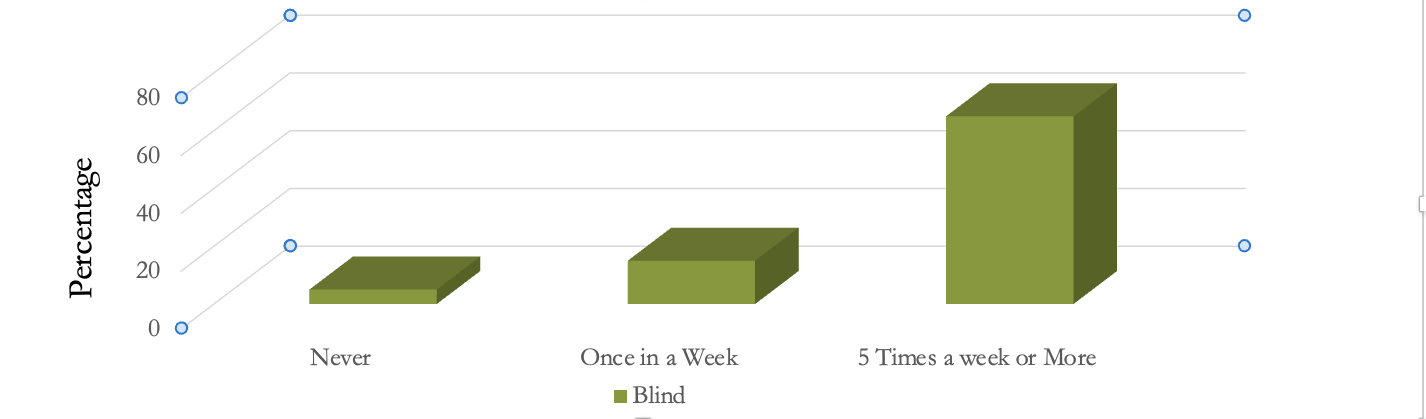
\includegraphics[width=0.95\textwidth]{Figures/Graph.png}
      \vspace{0.5em}
      \hrule
      \caption{\label{fig:including@a@picture}No.of Accidents per week vs Percentage }
      \vspace{0.5em}
      \hrule
   \end{figure}
\\
The data highlights the dire need for remedies to improve the security and health of those with visual impairments, as seen in Figure \ref{fig:including@a@picture}, which shows the amount of accidents each week vs the percentage. The graph shows the dangers they encounter on a daily basis.These difficulties can lead to a loss of independence and an increase in reliance on others. As a result, there is a need for an application that may help visually impaired people manage their daily lives more efficiently, allowing them to live more fulfilling lives with improved freedom and mobility. In essence, this project seeks to bridge the gap between the visually impaired community and the benefits of advanced technology. \\
\\
The program could change the way people live by answering their unique demands, from recognizing texts to obstacle identification, and by enhancing independence and flexibility.

\subsection{Sub-Problem}
\subsubsection{Text-Recognition}
\begin{enumerate}
\item \textbf{Problem Statement}
Text detection is the important component in the application, as the visually impaired individual cannot read a sign or a direction given on the boards or on signals. The text detection mechanism should be able to read in all text sizes and orientations and the accuracy should be more than 50 percent. Also the text detection should be conducted via video and give the user a real time feedback through the audio in the application.
\item \textbf{Methodology}
The model used in this was a Default Google ML-Kit text detection model which was easy to integrate in the application via Android Studio. The model is a pre-trained model which processes the video input coming through user's Mobile device with the help of 'Stream Mode' in the model's algorithm.
\item \textbf{Implementation}
Text-Recognition was successfully implemented with the help of ML-Kit Text detection model. The application was tuned by using algorithms for speed, taking advantage of machine acceleration when available, to guarantee real-time processing.\\
\\During implementation, the application encountered issues with image correctness, particularly when dealing with text on complicated backdrops and at varied scales. We addressed these issues by augmenting data, adjusting parameters, and testing with various CNN algorithms.
\end{enumerate}

\subsubsection{Object-Recognition}
\begin{enumerate}
    \item \textbf{Problem Statement}
    The object recognition sub-problem of the application is focused on the difficulty of allowing the application to reliably recognize and identify items throughout pictures acquired by the smartphone's lens. Identifying objects is an important function for those with visual impairments since it helps them recognize and communicate with what is around them. Yet, due to various particular obstacles, this activity is intrinsically difficult.
    Additionally, objects in the environment may be hard to identify since they may have similar shapes and sizes. The object detection model should be able to recognize these objects accurately even if they have similar visuals.
    \item \textbf{Methodology}
    To solve this problem, the application employed cutting-edge computer vision technologies and deep learning frameworks. The application used Convolutional Neural Networks (CNNs), a type of deep learning algorithm well-known for being able to thrive at image activities.
    The application has been implemented with A pre-trained tensorflow model named \textit{"SSD MobileNet"}. This model is trained to identify and recognise wide range of objects including cars, tables, chairs, truck, \textit{etc.}
    \item \textbf{Implementation}
    Application was tested using various models but only was used that was \textit{"SSD MobileNet"}. Understanding the significance of real-time object identification, the application has built improvements to guarantee that image pixels via the camera of the smartphone are processed quickly. For lowering processing load, parallel processing approaches, acceleration with the GPU, and model simplification were used. This functionality was tested under various conditions and lighting to ensure its adaptability.

\end{enumerate}
\subsubsection{Distance Calculation}
\begin{enumerate}
    \item \textbf{Problem Statement}
   This problem addresses the main obstacle of providing current data on the distance between the detected items and the user. This knowledge is critical for improving an individual's awareness of circumstances and guaranteeing secure movement, especially in potentially hazardous situations. The precision and accuracy of this feature is most important so it can give correct information to the user. It should provide approximate distance to the user so they can ensure their safety.

    \item \textbf{Methodology}
    Processing of the image through the \textit{"SSD Mobilenet"} model and finding the size and height of the object detected can be done with the help of processing the image. Distance estimation logic is implemented to calculate the approximate distance .
    \item \textbf{Implementation}
    The implementation of this functionality is a quite hard task. It requires accurate processing of the images and objects in the images. Sizes and heights of the object in the images is identified by image analysis. To attain real-time speed, the application enhance distance calculating methods for effectiveness. This guarantees that those using it receive instantaneous feedback on the proximity between objects and the user.



\end{enumerate}

\section{Tasks}

\subsection{Text-Recognition}
\subsubsection{Finding Right Model}
Choosing the best text-recognizing model is a critical step for the creation of the application. The model employed has a considerable impact on the precision as well as effectiveness of text identification among pictures. The text-recognition functionality has been experimented through a lot of model such as COCO datasets, You Only Look Once\textit{YOLOv4} Models, ML-Kit default Text Recognition model and Single Shot Detector\textit{SSD} MobileNet as well. This part looks into the method of determining the most appropriate approach for our text identification problem, taking seriously a variety of factors. The hunt for the most effective text recognition strategy started with a thorough examination of the current learning frameworks. The testing of all the pre-trained models was carried out in search of the best. ML-Kit's Default Text Recognition Model which excelled in performing best among all the model was further taken into consideration as the main model for Text Recognition. Finally, obtaining the best text-recognizing model required an in-depth procedure of architecture decision-making, significant information collecting, and enrichment.
\subsubsection{Real-Time Processing}
This task is focused to assuring that text detection and identification operate without significant delay, allowing people to receive text-based data from their surroundings immediately. Rapid processing is critical for visually impaired people because it improves their awareness of circumstance and enables them to engage with the environment more successfully. The models were also tested according to their processing of the detected text and how fast the text is detected. 
\begin{figure}[hbtp]
      \hrule
      \vspace{0.5em}
     \centering
      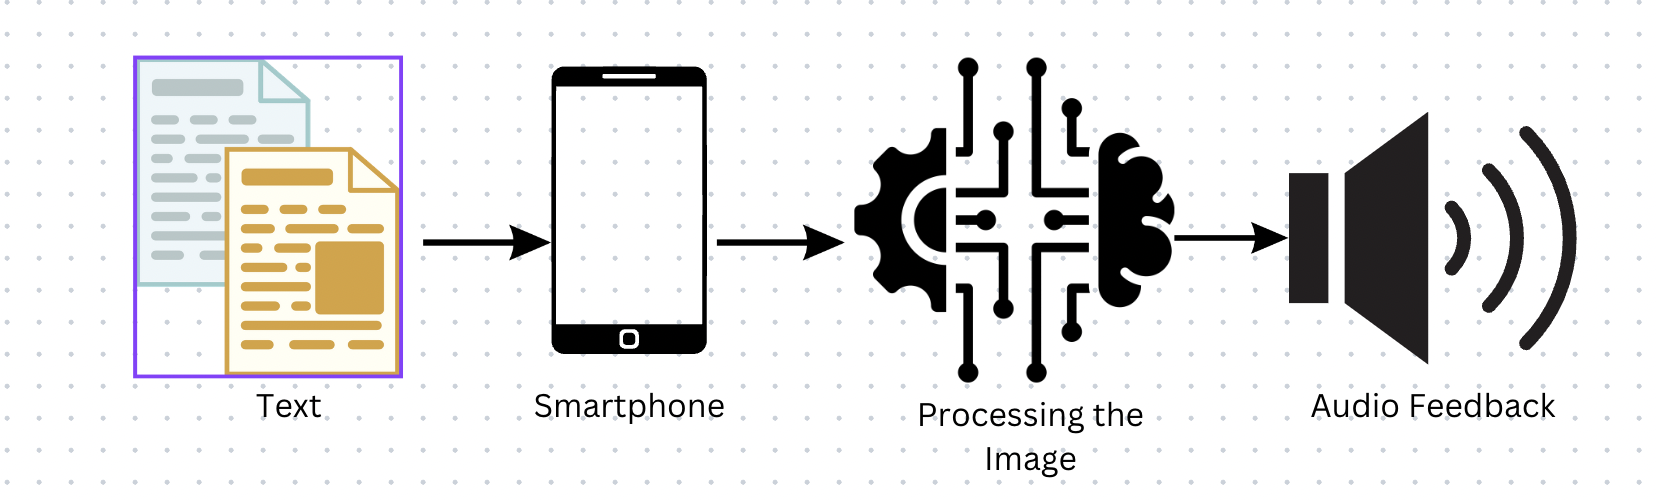
\includegraphics[width=0.95\textwidth]{Figures/task-TR.png}
      \vspace{0.5em}
      \hrule
      \caption{\label{fig:task-TR}Process for Text-Recognition }
      \vspace{0.5em}
      \hrule
   \end{figure}
   \\
To enable flawless immediate analysis, the application execute ongoing tracking of the video stream while the machine learning algorithm runs in the meantime. 
   
\subsection{Object-Recognition}
\subsubsection{Finding Right Model}
Finding the best algorithm for recognizing objects is an important part of designing the application since it affects its capacity to detect items and persons throughout pictures. Like text-recognition, the quest for the best recognition of objects model required careful thought and trial with several models. This part looks into the method of choosing the best solution to our object identification problem. The models which were looked at were Faster R-CNN, ML-Kit Object Detection Model, You Only Look Once\textit{YOLOv4} Models, and Single Shot Detector\textit{SSD} MobileNet as well. During the assessment phase, the computational models were rigorously evaluated with a variety of sets that included an extensive variety of items and situations frequently experienced by those with visual impairments. Finally, Single Shot Detector\textit{SSD} MobileNet model was selected.
\subsubsection{Real-Time Processing}
The software continuously records and analyses photos from the camera on the smartphone in real-time object identification, utilizing machine learning algorithms for recognizing items and humans. 
\begin{figure}[hbtp]
      \hrule
      \vspace{0.5em}
     \centering
      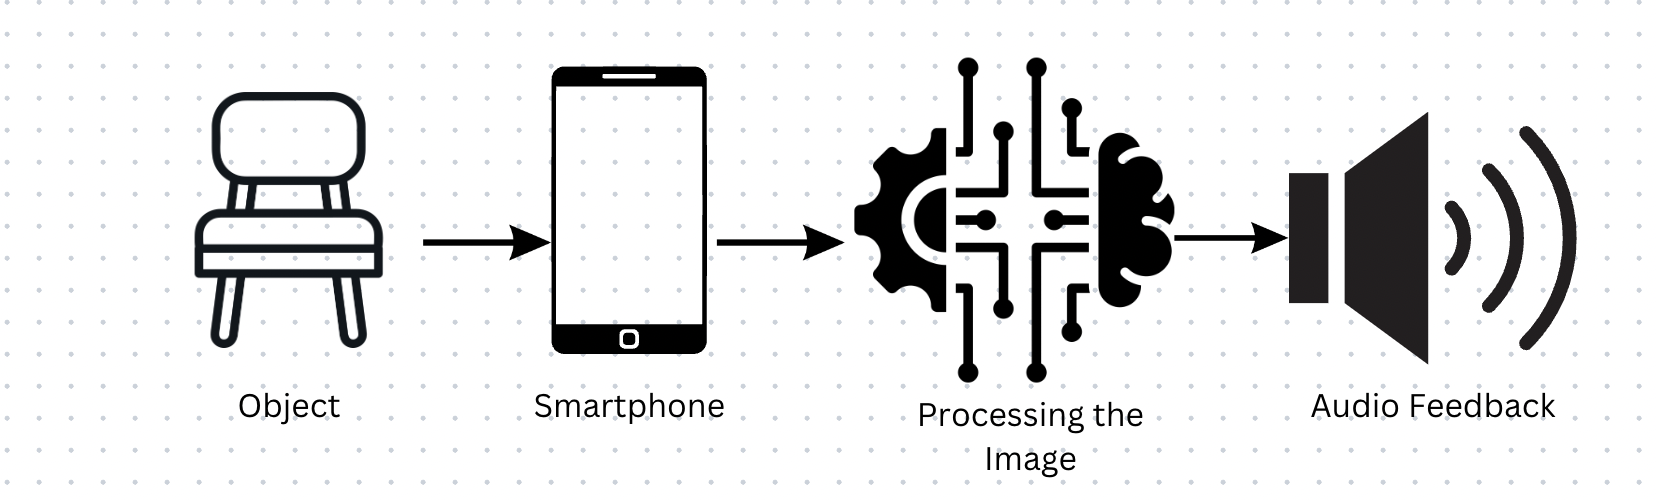
\includegraphics[width=0.95\textwidth]{Figures/task-OR.png}
      \vspace{0.5em}
      \hrule
      \caption{\label{fig:task-TR}Process for Object-Recognition }
      \vspace{0.5em}
      \hrule
   \end{figure}
   \\
To evaluate immediate processing, simulations are carefully evaluated on how well they're able to detect objects and persons in the viewer's field of vision in a timely manner. This includes assessing the thing identification system's velocity of processing, delay, and timing for responding. 

\subsection{Distance Calculation}
\subsubsection{Finding the Right Algorithm}

Finding the right algorithm for the distance estimation between the object and the user has its complexity. The program ran into a slew of techniques, all of which had its own set of benefits and drawbacks. But it arrived on an approach that achieves a compromise among precision and computing economy following extensive analysis and trial. Conventional computer vision approaches, including triangulation, that depend upon existing camera characteristics and measurement data, were investigated. Although these approaches can produce exact findings, they are frequently highly computational, which renders them unsuitable for use in real-time application. After searching and processing a lot of methods and techniques we arrived on formula which takes the inputs such as- Average of the real height of the object, Focal Length of the device in pixels and Object Height in Image. The formula is as follows:-\\
\\ \textbf{
\begin{math}Distance =   \big(Average Real Height of the Object  \times Focal Length in Pixels\big)    \div Object Height in Image
\end{math}}
                                              


\subsubsection{Real-Time Processing}
Finding the height of the object in the image and process is to get the distance is important to calculate the distance between the person and the object. There are a lot of algorithms to calculate the distance the implemented algorithm is precise and provides the user with distance in real-time. \begin{figure}[hbtp]
      \hrule
      \vspace{0.5em}
     \centering
      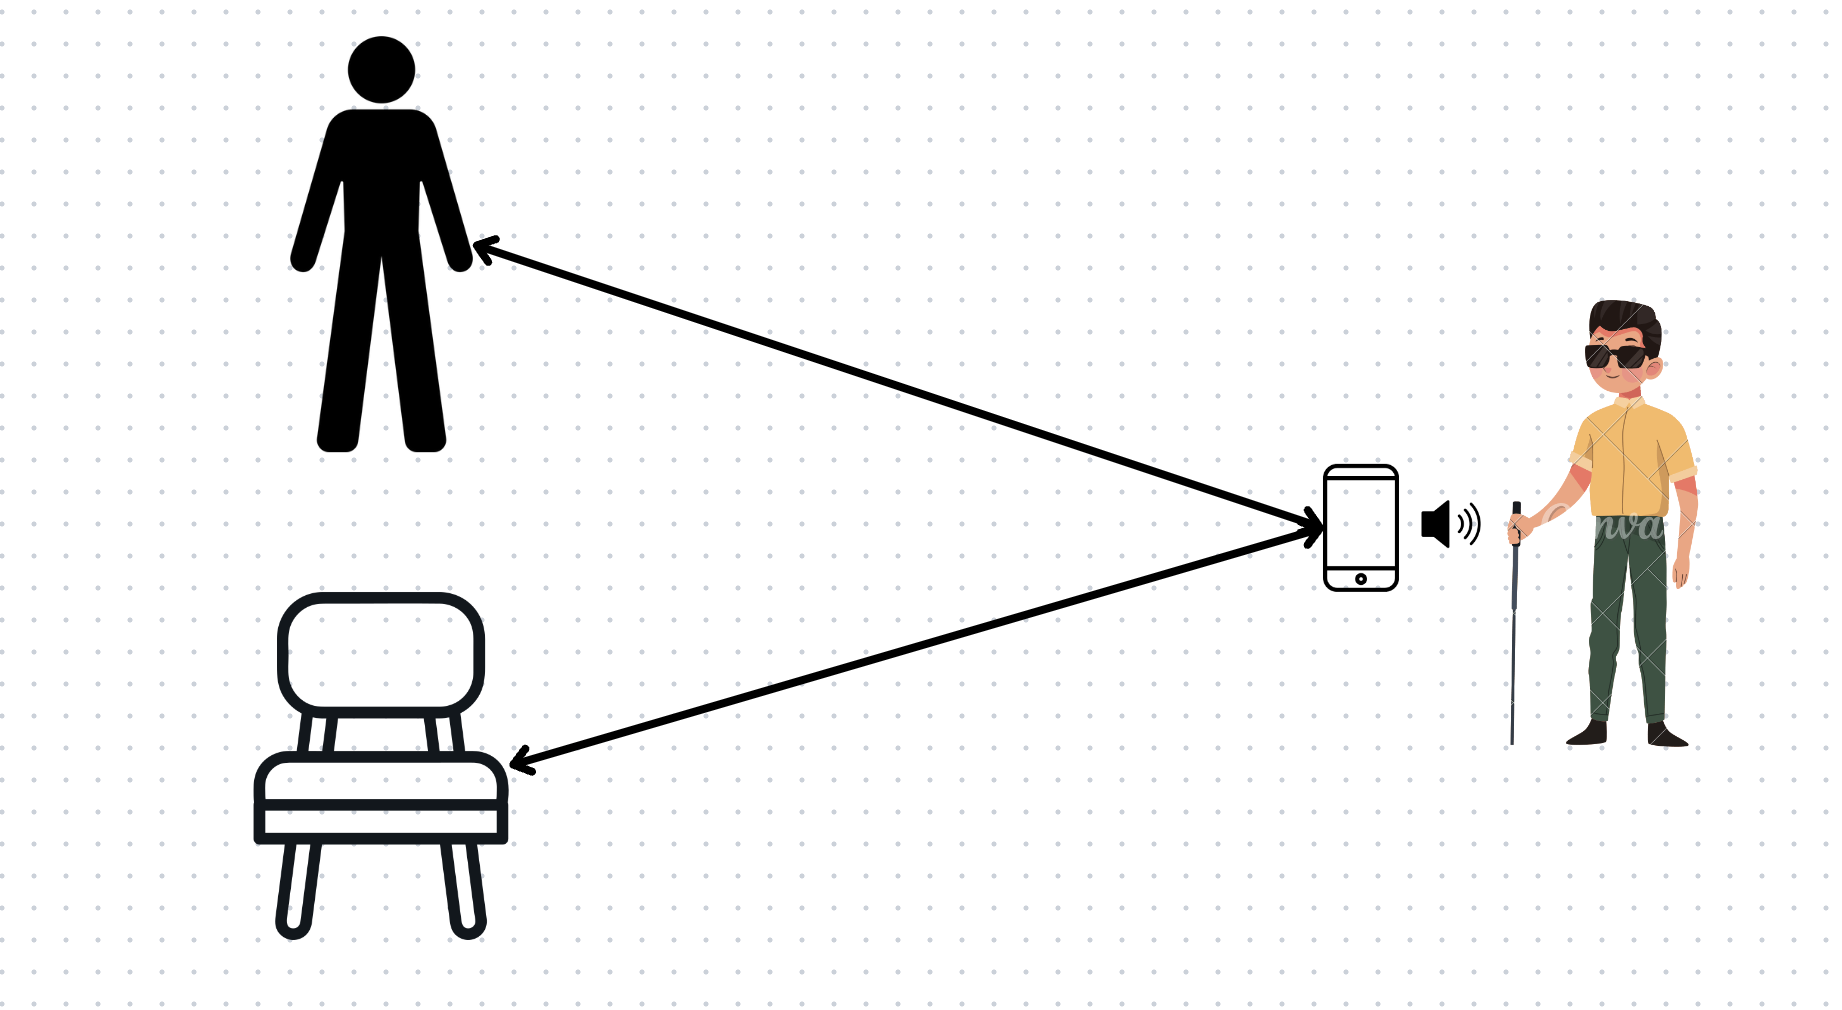
\includegraphics[width=0.95\textwidth]{Figures/distance.png}
      \vspace{0.5em}
      \hrule
      \caption{\label{fig:task-TR}Distance Evaluation }
      \vspace{0.5em}
      \hrule
   \end{figure}//The audio feedback is then provided to the user. This work entails continual evaluation of data and response production in order to offer individuals with accurate data, improving the security and trust as they traverse the world around them.



\section{Requirements}
\subsection{Functional Requirements}


\textbf{FR1:-}  The application should provide activities which can be used by the user
\\
\\\textbf{FR2:-}  The application should provide auditory confirmation when the user switches to any of the activity.
\\
\subsubsection{Activity For Text Recognition}

\textbf{FR3:-} The program ought to have a camera interface for taking text-filled pictures.
\\
\\\textbf{FR4:-} Text-to-speech technology should be used to translate the detected text into audible speech.
\\
\\\textbf{FR5:-} The process of text recognition should be started when a text is detected in the view of the user.
\\
\subsubsection{Activity For Object Recognition and Distance Measurement}

\textbf{FR6:-} The application should detect the objects using the device's camera.
\\
\\\textbf{FR7:-} The user should be given exposure to an audio description of the object's characteristics and features.
\\
\\\textbf{FR8:-} The camera should be able to be turned on by the user, who should also start the object detection procedure.
\\
\\\textbf{FR9:-} The distance between the identified item and the user should be displayed on the screen and communicated to the user audibly.
\\
\\\textbf{FR10:-} Object detection activity must detect a person.


\subsection{Non-Functional Requirements}

Non-functional requirements specify the qualities and limitations that outline how a system ought to function or operate. They are often referred to as quality attributes or system attributes. \\
\\
\textbf{NFR1:-} Users of all skill levels should have no trouble using all the pages because of the clear and simple user interfaces.
\\
\\\textbf{NFR2:-} The usage of flexible fonts and enough contrast between colours should be made 	to support individuals with visual disabilities.
\\
\\\textbf{NFR3:-} Minimum latency and nearly immediate response times should be characterised by all the pages
\\
\\\textbf{NFR4:-} Distance should be detected in a precise and on a real time basis
\\
\\\textbf{NFR5:-} The transition between activities ought to be seamless.

\section{Summary of Analysis Chapter}
The subject of the study, its related smaller issues, the activities required for dealing with these issues, and the crucial criteria that direct the growth of our dissertation topic were all thoroughly examined in this analysis chapter. We obtained a deeper grasp of the complex difficulties that our software seeks to address by breaking the problem down into its component sub-problems. The definition of certain duties shed light on the operational elements of our project and gave us an itinerary for execution. In addition, the definition of fundamental needs, including either functional and non-functional elements, forms the basis for the planning and creation of our project. This conceptual framework will play a crucial role as we move on with the succeeding stages of the project because it grounds our efforts in a methodical and knowledgeable approach to resolving the matter and attaining the intended outcomes.

\chapter{Design}
Our application's structure is deliberately created to maximize ease of use, usability, and user-centricity. The interface that we provide is developed with ease of use and effectiveness in consideration, allowing visually challenged people to move among the text recognition and object identification panels using touch commands. This chapter defines the design and the use cases of the application.
\section{User Interface}

\subsection{Text-Recognition Activity}
\begin{figure}[H]
      \hrule
      \vspace{0.5em}
     \centering
      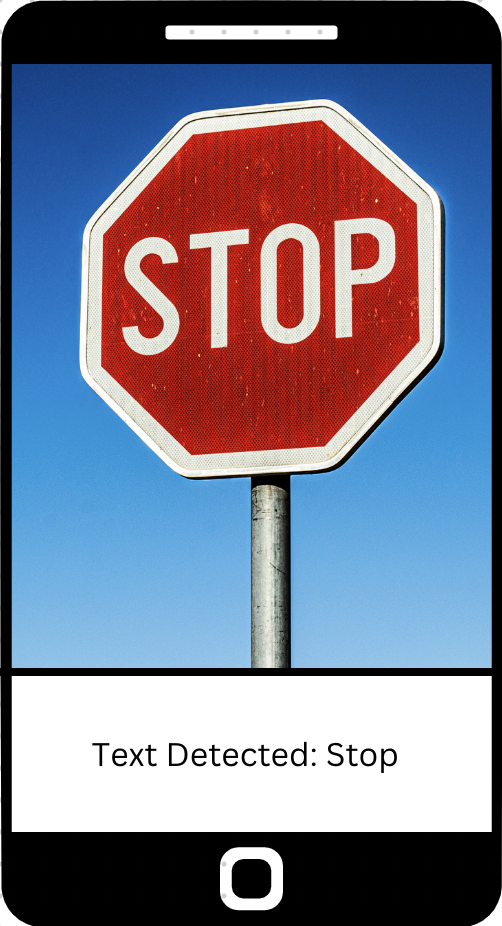
\includegraphics[width=0.29\textwidth]{Figures/TR-Activity.png}
      \vspace{0.5em}
      \hrule
      \vspace{0.5em}
      \caption{\label{fig:TR-Activity}User Interface for Text Recognition }
      \vspace{0.5em}
      \hrule
   \end{figure}

Elegance and usability are fundamental design concepts in the Text Recognition Activity's layout. Its design has been meticulously built to give those who are visually impaired with a smooth and straightforward interaction. As shown in the Figure \ref{fig:TR-Activity} a text box is given to describe the text and a auditory feedback is given whenever a text is appeared in the view of the smartphone's camera. The layout emphasizes the video feed, enabling individuals simply to direct the camera onto items or words they want to identify. The identified information is shown clearly on the screen in a readily apparent typeface. The user interface guarantees that recognised content is displayed in a user-friendly fashion, allowing users to quickly find and engage with the data.


\subsection{Object Recognition and Distance Measurement Activity}

The Object Identification Activity is an essential element in the setting of the application's graphical user interface, intended to promote smooth communication among those with visual impairments and its object recognition capability. This activity also provides the distance between the object and the user in the format of meters. This exercise has been carefully designed to promote availability, effectiveness, and simplicity, enabling users to easily leverage the potential of object identification.


\begin{figure}[H]
      \hrule
      \vspace{0.5em}
     \centering
      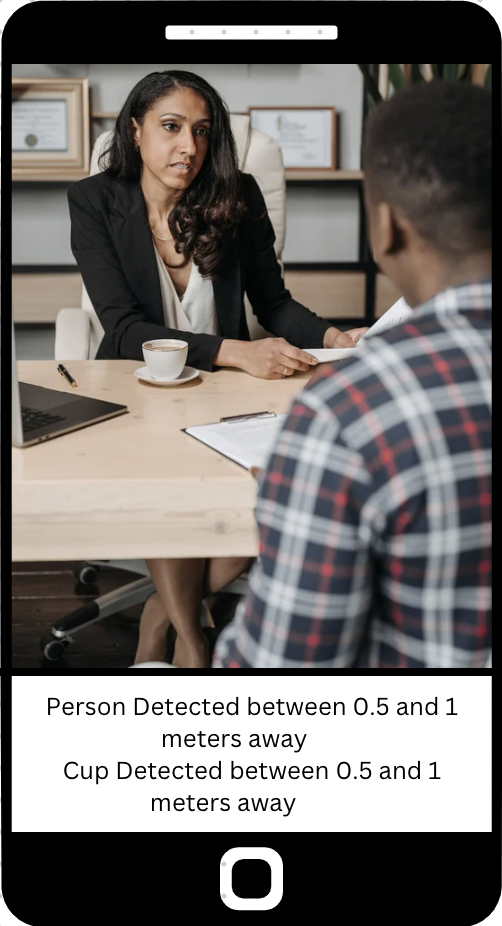
\includegraphics[width=0.35\textwidth]{Figures/OR-Activity.png}
      \vspace{0.5em}
      \hrule
      \vspace{0.5em}
      \caption{\centering\label{fig:OR-Activity}User Interface for Object Recognition and Distance Measurement Recognition }
      \vspace{0.5em}
      \hrule
   \end{figure}

A text box is given to provide clear interaction between the application and the user. To improve the user's attention on the job at the same direction, the design stresses clarity and eliminates distraction. This stream provides users with current insights into the world around them, guaranteeing that they acquire accurate and recent data regarding observed items and individuals. The video feed is incorporated smoothly into an intuitive interface, providing users with a live and interactive picture of their surroundings. The distance is provided for a lot of objects including Chair, Cup, Person, Table, \textit{etc.} 

\subsection{Screen Switching}

The inclusion of screen switching, which allows individuals to effortlessly shift among two critical screens: the text recognition screen and the object detection screen, is a fundamental part of the user interface. The screen changing mechanism had been meticulously created to allow people with normal eyesight to effortlessly navigate the application. When engaging with the application through touch, users may easily move between the text identification and object detection interfaces.

\begin{figure}[H]
      \hrule
      \vspace{0.5em}
     \centering
      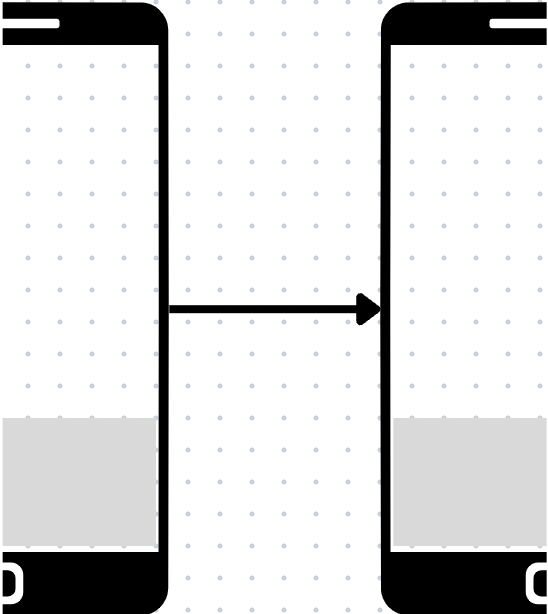
\includegraphics[width=0.35\textwidth]{Figures/Screen Switch.png}
      \vspace{0.5em}
      \hrule
      \vspace{0.5em}
      \caption{\centering\label{fig:SS}Screen Switching Mechanism}
      \vspace{0.5em}
      \hrule
   \end{figure}
   In overall, the display shifting design of the user interaction is targeted on maximizing the app's accessibility for vision challenged users. We hope to develop a layout that allows users to fully utilize the functionality of our program by combining straightforward navigation, aural input, and centered around users design concepts.



   \section{UML Diagram}

   \subsection{Class Diagram}
   A Class Diagram is an important part of the Unified Modeling Language (UML), which is utilized in computer science and system development. It is a diagram of a method's structural form, focused on categories, their characteristics, methods, and the interactions among them.

   The following Diagram depicts all the attributes and the methods inside of the classes of our application.
\begin{figure}[H]
      \hrule
      \vspace{0.5em}
     \centering
      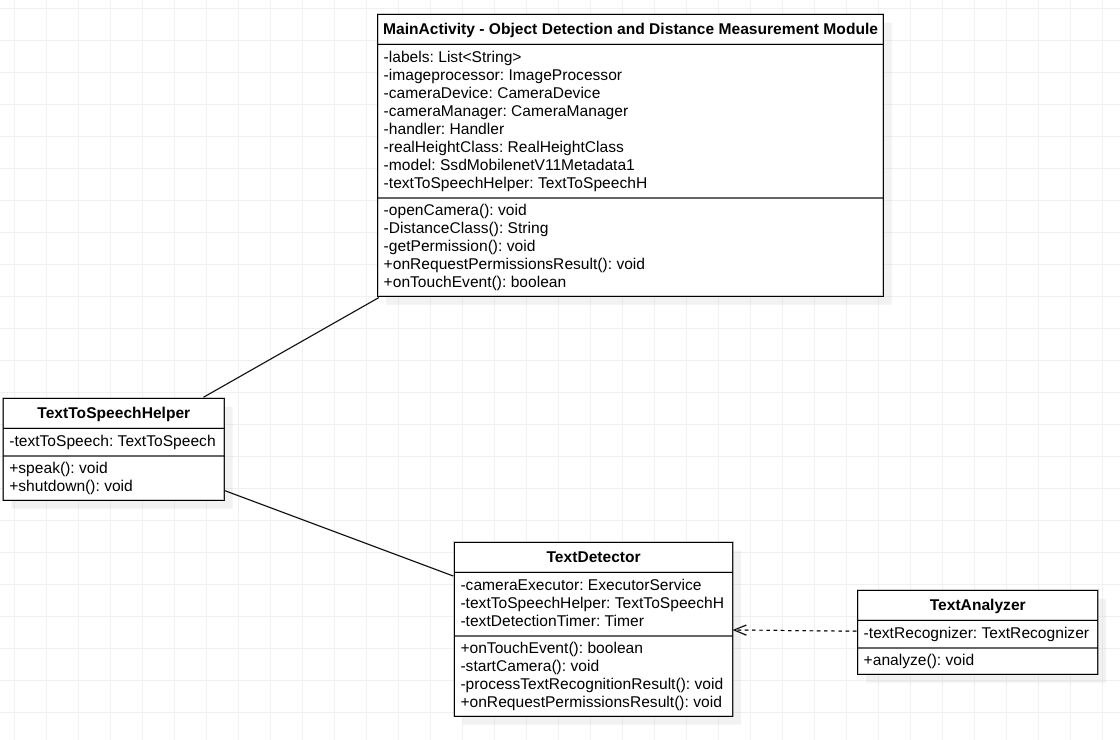
\includegraphics[width=0.9\textwidth]{Figures/ClassDiagram.png}
      \vspace{0.5em}
      \hrule
      \caption{\centering\label{fig:CD}Class Diagram}
      \vspace{0.5em}
      \hrule
   \end{figure}

 As shown in the Figure \ref{fig:CD} the main class of the application is Object Recognition and Distance Evaluation. Both the Object Recognition and Distance Evaluation class and Text Detector class inherits Text to Speech helper class which handles the auditory output of the application. The TextAnalyzer class is the class inside of the TextDetector class which analyze method which processes the input live feed which is coming from the user's smartphone.


   \subsection{Sequence Diagram}
   A sequence diagram is a sort of Unified Modeling Language (UML) graph utilized in computer science and system architecture to depict the relationship and succession of signals passed among entities or elements in an infrastructure or software program. Diagrams of sequences are especially effective for describing a system's fluid behavior, since they show that multiple pieces of the whole work together to attain certain capability.
   \newpage
   \subsubsection{Text Recognition}
   The sequence diagram for Text Recognition Activity is as follows:- 
   \begin{figure}[H]
      \hrule
      \vspace{0.5em}
     \centering
      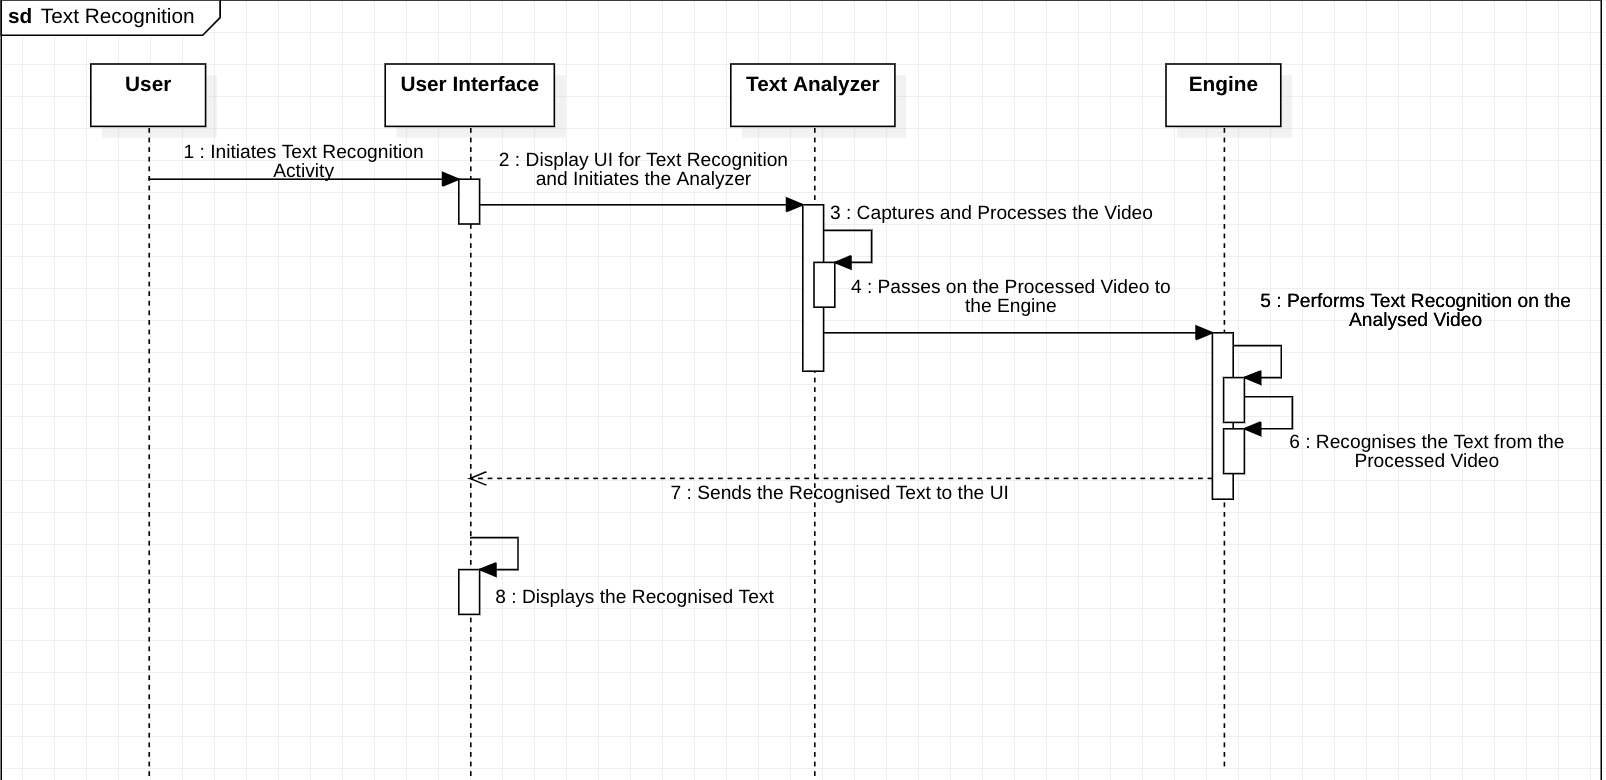
\includegraphics[width=0.9\textwidth]{Figures/TR-SD.png}
      \vspace{0.5em}
      \hrule
      \caption{\centering\label{fig:TR-SD}Text Recognition Sequence Diagram}
      \vspace{0.5em}
      \hrule
   \end{figure}

   In the Figure \ref{fig:TR-SD}:
\begin{enumerate}
    \item A text recognition action is started by the user.
    \item The User Interface presents the text recognition graphical user interface.
    \item The User Interface loads the video.
    \item UI sends the video to the analyzer 
    \item Text Analyzer processes the video and passes the processed video to the engine.
    \item The engine recognises the text from the video with the help of the text detection model and sends it back to the UI.
    \item UI displays the recognised text.
\end{enumerate}
\newpage
\subsubsection{Object Recognition and Distance Measurement}
The sequence diagram for Object Recognition and Distance Measurement Activity is as follows:- 
\begin{figure}[H]
      \hrule
      \vspace{0.5em}
     \centering
      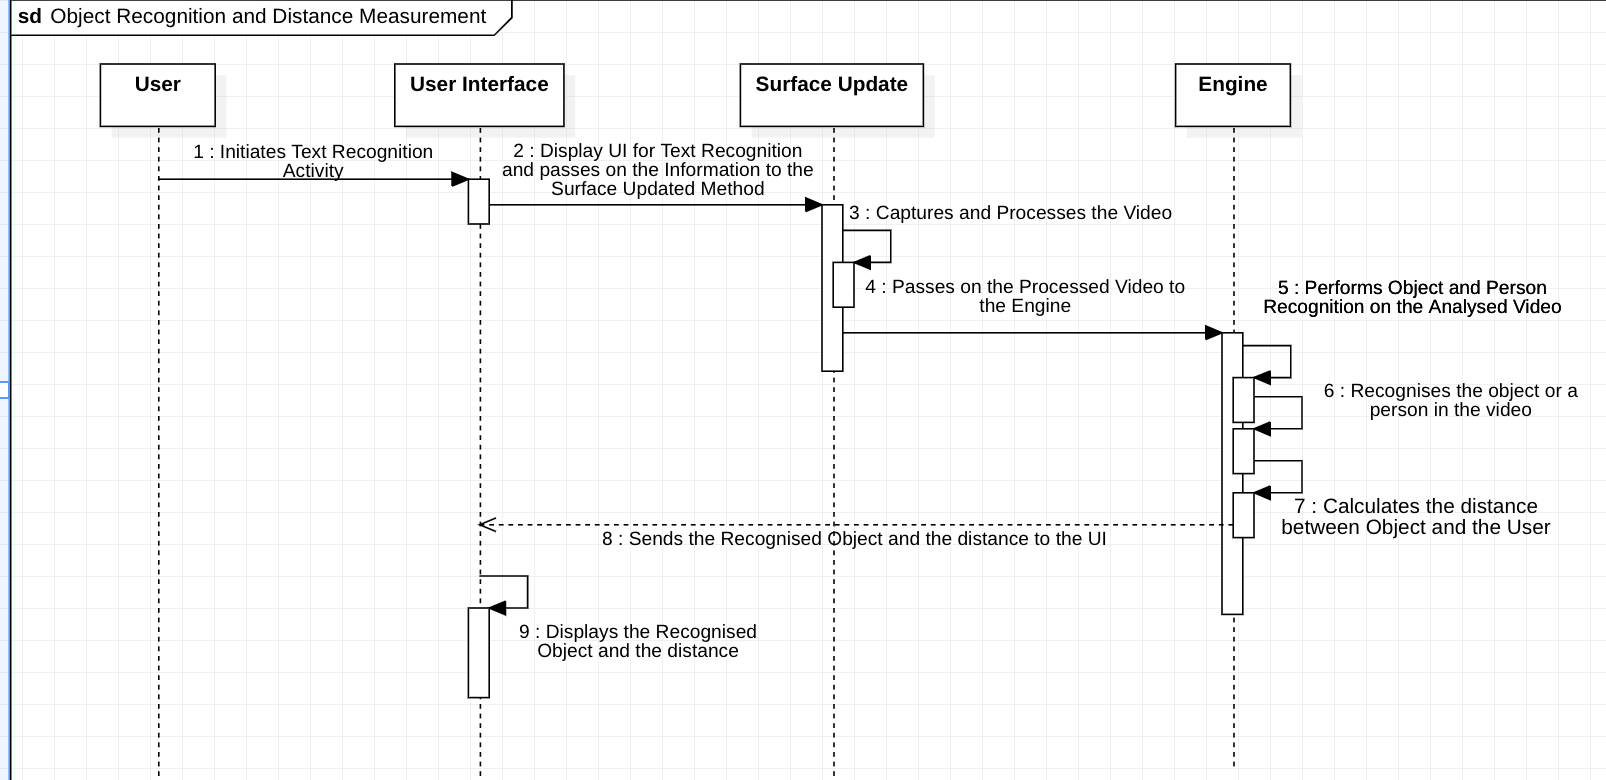
\includegraphics[width=0.9\textwidth]{Figures/OR-SD.png}
      \vspace{0.5em}
      \hrule
      \caption{\centering\label{fig:OR-SD}Object Recognition and Distance Measurement Sequence Diagram}
      \vspace{0.5em}
      \hrule
   \end{figure}

   In the Figure \ref{fig:OR-SD}:
   \begin{enumerate}
    \item Object recognition action is started by the user.
    \item The Object Recognition graphical user interface is displayed in the User Interface.
    \item The User Interface loads the video.
    \item UI sends the video to the Texture View's OnSurfaceUpdated method
    \item OnSurfaceUpdated processes the video and passes the processed video to the engine.
    \item The engine recognizes the object and the distance to the object from the user using the object detection model and distance measurement method and returns it to the user interface.
    \item UI displays the recognised object and the distance.
\end{enumerate}


\section{Back-end}

The Back-end of the application consist of the powerful technologies such as ML KIT and Tensorflow. This frameworks are selected very strategically keeping in mind the the app's response time, accessibility and performance.
MLKit Text Detection Model and \textit{Single Shot Detector}(SSD) Mobile Net model has been implemented as the back-end models for this application.


\subsection{ML Kit}
ML Kit's default Text Recognition model has been seamlessly integrated in the back-end of the application. It provides models that have been trained and makes it easier to build features like word recognition, picture categorizing, and recognizing objects. We used only the model for the text recognition in this application. The user-friendliness and the model's accessibility is the main reason for this usability. 
\begin{wrapfigure}{r}{0.4\textwidth}
\centering
    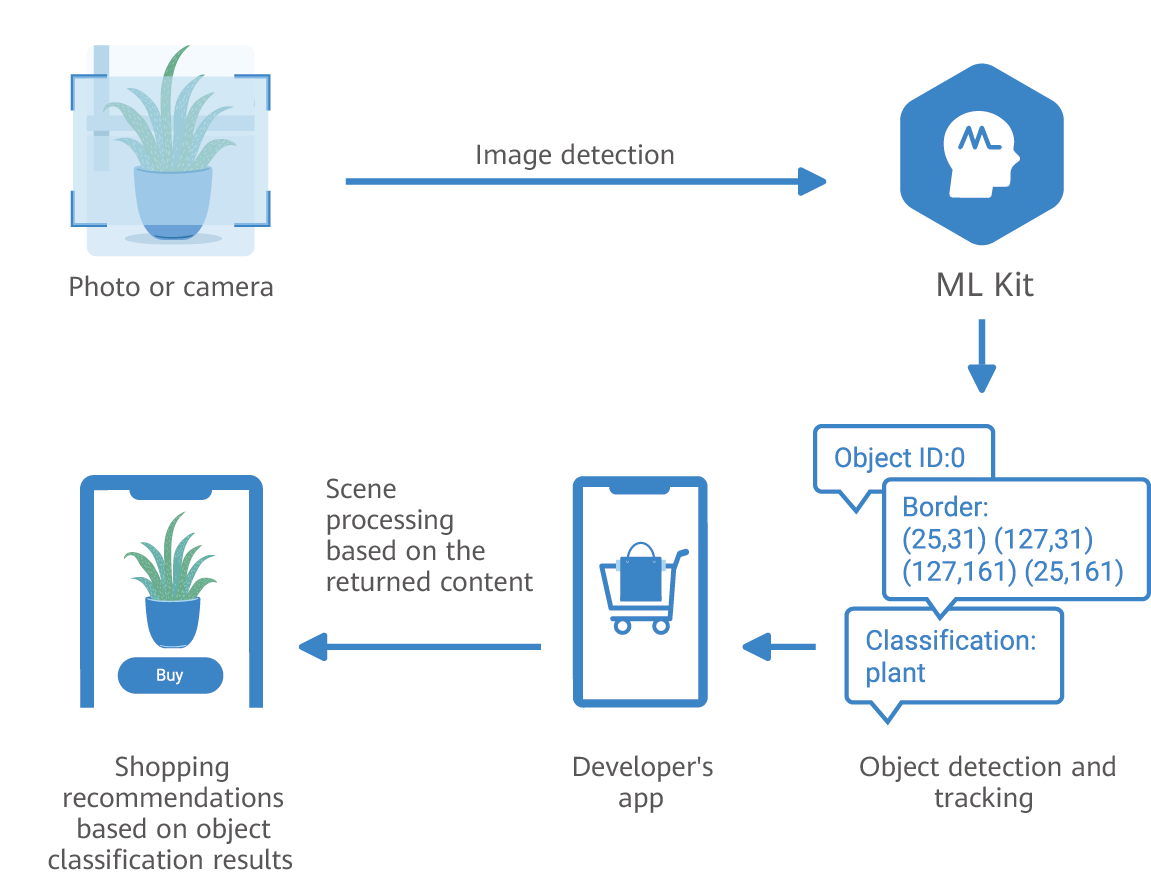
\includegraphics[width=0.5\textwidth]{Figures/mlkit-ex.png}
    \caption{\centering ML-KIT Recognition process}
    \label{fig:mlkit-ex}
\end{wrapfigure}
As shown in the Figure \ref{fig:mlkit-ex} the process of the recognition of the object or the text in ML-Kit's model is complex. ML-Kit provides the simplest model integration methods. It takes the image or a video feed into as the data input and processes them by resizing the image. It classifies the objects based on the size or the shape of the object. For example, if the image consist of chair it will first pre-process the image and then match the shape and colour of the object in the image with the data which is their in the model. It then returns the output in the form of labels or text. 
ML-Kit has been directly combined in the application with the help of Android Studio's dependencies. ML-Kit dependencies used in this applications are:- 
\begin{enumerate}
    \item 'com.google.android.gms:play-services-mlkit-text-recognition-common:19.0.0'
    \item 'com.google.android.gms:play-services-mlkit-text-recognition:19.0.0'

\end{enumerate}
Both of the dependencies serves as the basis for automated text recognition activities and can contain common algorithms and assets needed by several text recognition capabilities. These dependencies are helpful in extracting the text from an image and sending the text to the user interface.

\subsection{TensorFlow}

The TensorFlow's \textit{Single Shot Detector}(SSD) MobileNet Model has been implemented for the Object Detection Function of the Application. It consists of a pair of primary parts: MobileNet for the extraction of features and the Single Shot MultiBox Detector (SSD) for identifying an object. SSD MobileNet models are frequently initially trained on enormous databases that include COCO (Common Objects in Context) or Pascal VOC. Android Studio only uses \textit{".tflite"} tensor flow models. The model is added in the ml directory of the application and the the following dependency is then added to the application \textit{"org.tensorflow:tensorflow-lite:2.5.0"}\\

\begin{figure}[H]
      \hrule
      \vspace{0.5em}
     \centering
      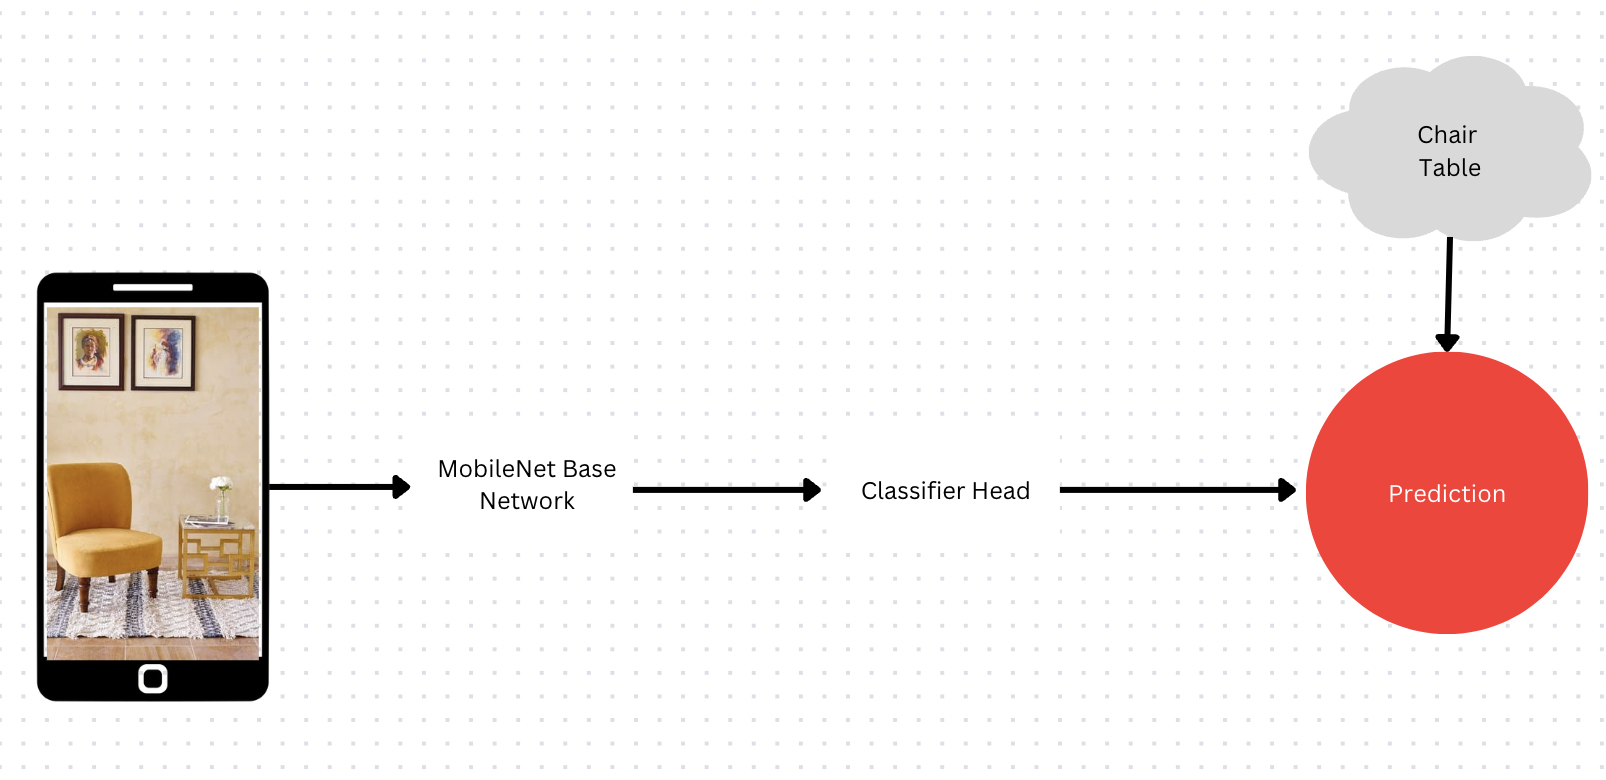
\includegraphics[width=0.8\textwidth]{Figures/SSD.png}
      \vspace{0.5em}
      \hrule
      \caption{\centering\label{fig:SSD}SSD MobileNet Architecture}
      \vspace{0.5em}
      \hrule
   \end{figure}

MobileNet is a convolutional neural network (CNN) design designed specifically for devices that are mobile or embedded. It provides the foundation for the SSD MobileNet approach, extracting characteristics from raw photos. SSD MobileNet makes use of numerous feature representations with varying spatial levels. Multiple components in the MobileNet framework build such map representations. 


\section{Flow Chart Of System Architecture}
\begin{figure}[H]
      \hrule
      \vspace{0.5em}
     \centering
      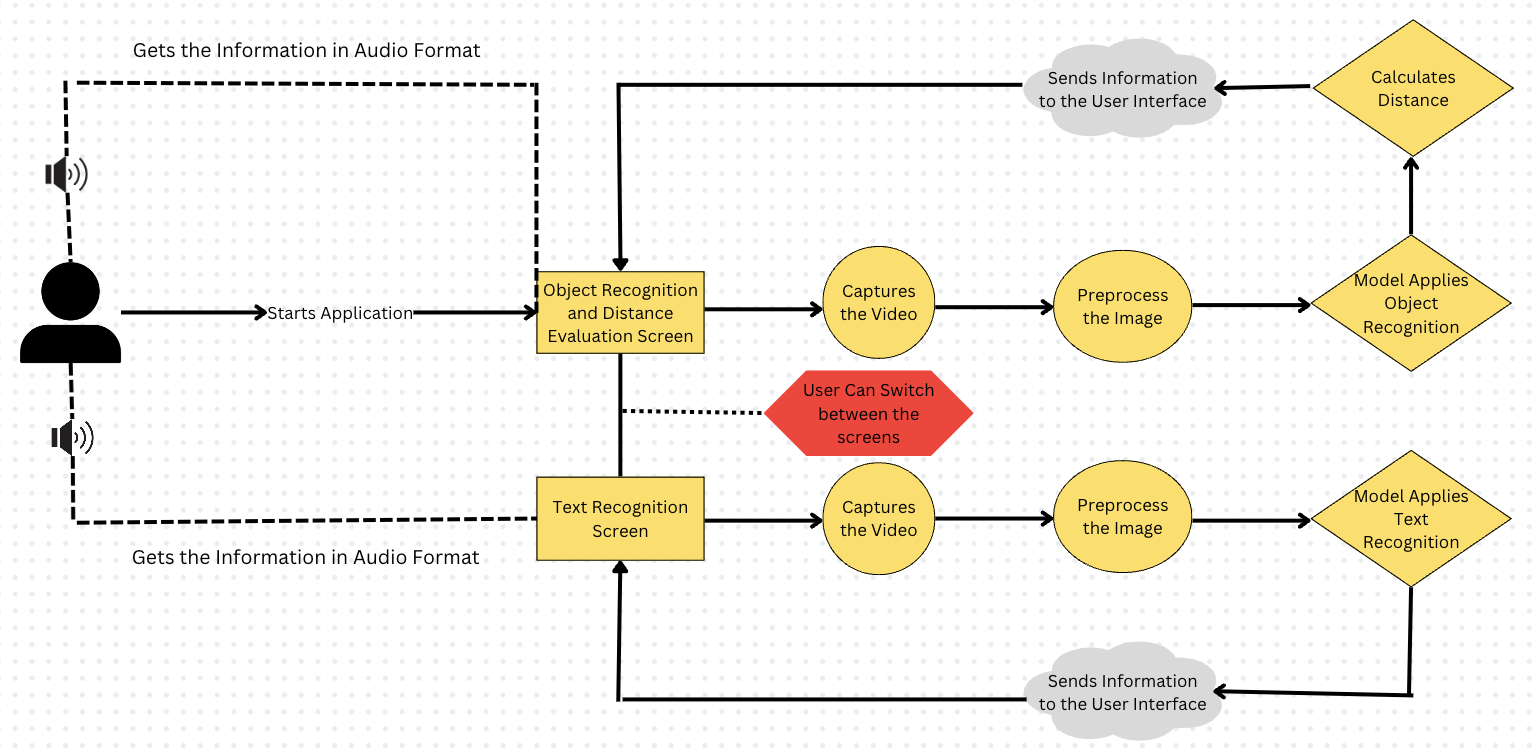
\includegraphics[width=1\textwidth]{Figures/SystemDesign.png}
      \vspace{0.5em}
      \hrule
      \caption{\centering\label{fig:SystemDesign}System Architecture}
      \vspace{0.5em}
      \hrule
   \end{figure}

Above Figure shows how the application works and how it provides auditory feedback to the user. The User starts the application and the first screen that the application shows is the Object Recognition And Distance Evaluation Screen-MainActivity. The user can either switch to the Text Recognition Screen by swiping to the right or stay on the First screen itself, depends on the user's choice. Whenever the screen switches it provides auditory confirmation of the user's screen. For Example, if the user is on Text Recognition Screen it says \textbf{"Text Mode On"}. The user then faces the smartphone camera towards the environment and depends on which mode is on the application detects the objects or texts.  The Object Detection can identify Person, Objects and can also determine distance between the user and them. Object and Text Recognition models processes the image by resizing them and then the model applies the feature extraction on the video so it can detect the objects and text in real time. The information is then passed on to the user interface and the application also provides the information to the user in auditory format.


\section{Summary of Design Chapter}
We have thoroughly examined the creation stage and not just explained the complex workings of our program, but also demonstrated its usefulness and sturdiness. The presentation of many displays, namely the text identification and recognizing objects screens, showed off their user-friendly interfaces and smooth transition capabilities. The usage of UML diagrams, such as sequence diagrams, and class diagrams, gave our application's operation an organized design while emphasizing the key interactions and parts. In addition, a full description of the information flow procedures and back-end architecture highlighted the technological foundations enabling an intuitive user experience. As we arrive at the end of this design chapter, it is clear that the careful design decisions and technical demands we made set a solid basis for the resulting development and assessment phases, announcing an application that not only satisfies user needs but also illustrates creative thinking and availability in the field of technological assistance.



\chapter{Implementation}

This chapter delves deeper into the Application's implementation. The development of the application's topics of concern, in addition to a few of the more complicated steps and procedures, are examined and described extensively.

\section{Camera Integration}
\subsection{Camera Permission}
\begin{scriptsize}
    \begin{verbatim}
        private void getPermission() {
        if (ContextCompat.checkSelfPermission(this, Manifest.permission.CAMERA) != 
        PackageManager.PERMISSION_GRANTED) {
            if (Build.VERSION.SDK_INT >= Build.VERSION_CODES.M) {
                requestPermissions(new String[]{Manifest.permission.CAMERA}, 101);
            }
        }
    }
    \end{verbatim}
\end{scriptsize}
The code for getting the camera permission from the manifest is done in the above code. It displays how it checks the permission is granted or not with the help of \textit{checkSelfPermission} and if permission is not granted it displays a alert so that the user can choose to grant a permission or not.
\subsection{Starting and Setting up Image Analysis}
Initialisation of the camera is done by the startcamera() method. All the camera related functionalities is done in this method. It is as follows:
\begin{scriptsize}

\begin{verbatim}
    private void startCamera() {
        // Get an instance of ProcessCameraProvider
        ListenableFuture<ProcessCameraProvider> cPF =
        ProcessCameraProvider.getInstance(this);
        cPF.addListener(() -> {
            try {
                // Get the ProcessCameraProvider object
                ProcessCameraProvider cP = cPF.get();

                Preview preview = new Preview.Builder().build();
                preview.setSurfaceProvider(previewView.getSurfaceProvider());

                ImageAnalysis iA = new ImageAnalysis.Builder()
                        .setBackpressureStrategy(ImageAnalysis.STRATEGY_KEEP_ONLY_LATEST)
\end{verbatim}
\end{scriptsize}

 The above code displays initializing the camera and then using the variable to start the instance. The CameraX library is used in this application to engage and use the camera-related tasks.
The startCamera() operation in the mobile application sets up the digital camera capability. It starts by acquiring a ProcessCameraProvider instance, that is a critical component of CameraX. This service source grants connectivity to the camera's capabilities. Preview view is used to better integrate withe the CameraX library. It then configures an ImageAnalysis function with a custom TextAnalyzer.

\begin{scriptsize}
    \begin{verbatim}
        iA.setAnalyzer(cameraExecutor, new TextAnalyzer());

                CameraSelector cS = new CameraSelector.Builder()
                        .requireLensFacing(CameraSelector.LENS_FACING_BACK)
                        .build();

                cP.bindToLifecycle((LifecycleOwner) this, cS, 
                preview, iA);
                preview.setSurfaceProvider(previewView.getSurfaceProvider());
            } catch (ExecutionException | InterruptedException e) {
                Log.e(TAG, "Error starting camera: " + e.getMessage());
            }
        }, ContextCompat.getMainExecutor(this));
    }
    \end{verbatim}
\end{scriptsize}

The above code is the continuation of startcamera(). It configures numerous camera applications via the addListener() function. It starts by creating a Preview instance and setting it for showing the image from the camera's preview view on a specific previewView. Users may view everything the camera's sensor is collecting in the moment.  This use case records camera pixels and sends these to the TextAnalyzer for text recognition. Binding the use case is done with the help of 'cameraProvider.bindToLifecycle()'


\section{Sliding Animation}
The user can switch between the two screens with the help of the following code:-
\begin{scriptsize}
    \begin{verbatim}
        public boolean onTouchEvent(MotionEvent tE){
        switch (tE.getAction()){
            case MotionEvent.ACTION_DOWN:
                a1=tE.getX();
                b1=tE.getY();
                break;
            case MotionEvent.ACTION_UP:
                a2=tE.getX();
                b2=tE.getY();
                if(a1>a2){
                    Intent intent1=new Intent(MainActivity.this, TextDetector.class);
                    startActivity(intent1);
                    overridePendingTransition(R.anim.sliderighti, R.anim.slidelefto);
                }else if(a1<a2){
                    Intent intent2=new Intent(MainActivity.this, TextDetector.class);
                    startActivity(intent2);
                    overridePendingTransition(R.anim.slidelefti, R.anim.sliderighto);
                }
                break;
        }
        return false;
    }
    \end{verbatim}
\end{scriptsize}
 The 'onTouchEvent' method is generally used to manage all the touch events on the android device. The Switch method is used to handle the motion events such as ACTION-UP and ACTION-DOWN. ACTION-DOWN event is when the user touches the screen and both the coordinates are obtained by touchEvent.getX() and touchEvent.getY() and for the ACTION-UP is when the user user removes the hand from the screen. The conditions are checked to determine whether the user slide the screen from right to left or left to right. In this case the the code is written in such a way that it does not matter if the user slides to the left or to the right, the screen will definitely go to the other activity as there are only two screens. The method overridePendingTransition() is a in-build method to perform the animation on the given screens.

 \section{ML-Kit Model Integration}
 The following snippet provides the code for integration of ML-Kit's Default Text Recognition Model.
 
 \begin{scriptsize}
     \begin{verbatim}

private class TextAnalyzer implements ImageAnalysis.Analyzer {
        private TextRecognizer textRecognizer;
        private boolean isTextRecognized = false;

        @Override
        @ExperimentalGetImage
        public void analyze(@NonNull ImageProxy iP) {
            
            if (!isTextDetectionAllowed) {
                iP.close();
                return;
            }

            Image mI = iP.getImage();

            if (mI != null) {
                // Create an InputImage from the media Image
                InputImage iI = InputImage.fromMediaImage(mI,
                iP.getImageInfo()
                .getRotationDegrees());
                     \end{verbatim}
 \end{scriptsize}

 The TextAnalyzer class is essential for initializing the text recognizer object and performing text recognition methods on the image. It uses the default options provided by TextRecognizerOptions.DEFAULTOPTIONS. The analyze method is used to get the image with the help of image proxy instance in the Image object.
 \begin{scriptsize}
     \begin{verbatim}
     // Process the input image using the TextRecognizer
                textRecognizer.process(iI)
                        .addOnSuccessListener(new OnSuccessListener<Text>() {
                            @Override
                            public void onSuccess(Text text) {
                                processTextRecognitionResult(text);
                                iP.close();
                            }
                        })
                        .addOnFailureListener(new OnFailureListener() {
                            @Override
                            public void onFailure(@NonNull Exception e) {
                                Log.e(TAG, "Text recognition error: " + e.getMessage());
                                iP.close();
                            }
                        });
            
         
     \end{verbatim}
 \end{scriptsize}

This Image object is then stored in the InputImage variable with additional information such as image degrees. If the textrecognizer object is successful in processing the image it goes to processTextRecognitionResult method with the help of onSuccessListener. And if the textrecognizer object is unsuccessful it returns the error in the Log and closes the imageproxy.\\
The processTextRecognitionResult method is as follows: 

 \begin{scriptsize}
     \begin{verbatim}
         private void processTextRecognitionResult(Text text) {
        
        int wordsDetected = 0;
        for (Text.TextBlock block : text.getTextBlocks()) {
            for (Text.Line line : block.getLines()) {
                String[] words = line.getText().split("\\s+");
                for (String word : words) {
                    recognizedText.append(word).append(" ");
                    wordsDetected++;
                    if (wordsDetected >= maxWordsToDetect) {
                        break; // Break the loop if the maximum words limit is reached
                    }
                }
                if (wordsDetected >= maxWordsToDetect) {
                    break; // Break the loop if the maximum words limit is reached
                }
            }
            if (wordsDetected >= maxWordsToDetect) {
                break; // Break the loop if the maximum words limit is reached
            }
        }
        \end{verbatim}
 \end{scriptsize}
 The above code gets the text from the processor and gets it together using append. The method also tells the system when to stop the detection and when to start again. The maximum limit to detect the words is also set to 10 words so that the detection object should detect only 10 words at one detection

 \begin{scriptsize}
     \begin{verbatim}
         textDetectionTimer.schedule(new TimerTask() {
            @Override
            public void run() {
                isTextDetectionAllowed = true;
            }
        }, 5000);
     \end{verbatim}
 \end{scriptsize}
The above code if for the text detection timer which presents the number of seconds it will take to detect the text after one round of detection.

\begin{scriptsize}
    \begin{verbatim}
    // Get the new text and check if it's significantly different from the previous text
        final String newText = recognizedText.toString().trim();
         // Modify the length requirement as needed
            runOnUiThread(() -> {
                TextView textView = findViewById(R.id.text_view);
                if (newText.isEmpty()) {
                    textView.setText(""); // Clearing the TextView if there is no text
                } else {
                    textView.setText("Text Detected: " + newText);
                    textView.setMaxLines(5); // Set maximum number of lines to 1
                     // Add ellipsis at the end if text is too long
                    textToSpeechHelper.speak("Text Detected: " + newText);
                }
            });
    
        
    \end{verbatim}
\end{scriptsize}
        
The above code sends the detected text to the textview via newText variable and sets the string attached to it. If newText is empty, textview.setText("") clears the text content of the TextView by setting it to an empty string, effectively removing any previously displayed text. The "textView.setMaxLines(5)" line limits the TextView to displaying a maximum of 5 lines of text. If the detected text is longer than 5 lines, it will be truncated, and an ellipsis (...) will be added to indicate that there is more text.


\section{TFlite SSD MobileNet Integration And Distance Evaluation}

The code for integrating ML-Kit's Default Text Recognition Model is provided in the following excerpt.

\begin{scriptsize}
    \begin{verbatim}
private SsdMobilenetV11Metadata1 model;
try {
            model = SsdMobilenetV11Metadata1.newInstance(this);
            labels = FileUtil.loadLabels(this, "labels.txt");
        } catch (IOException e) {
            e.printStackTrace();
        }

iP = new ImageProcessor.Builder().
add(new ResizeOp(300, 300, ResizeOp.ResizeMethod.BILINEAR)).build();

 \end{verbatim}
\end{scriptsize}

'SsdMobilenetV11Metadata1' is initialised and used in this code. It uses FileUtil.loadLabels() to obtain names using a text file called "labels.txt" to categorize observed items. Image processor object is created to preprocess the image and resize the image into 300x300 via Resizeop method.

\begin{scriptsize}
    \begin{verbatim}
        handler.post(new Runnable() {
                    @Override
                    public void run() {

                        StringBuilder detectedObjectsBuilder = new StringBuilder();
                        bitmap = textureView.getBitmap();
                        TensorImage image = TensorImage.fromBitmap(bitmap);

\end{verbatim}
\end{scriptsize}

The Handle run() method does all the work. A Handler is a mechanism for running code on the UI thread from a different thread.  It obtains the bitmap from the textureview of the appliaction to process the captured image and convert it to the TensorImage. A textureView is a view in Android that can display a bitmap or video stream, often used for camera previews or rendering graphics. Applying the fromBitmap method, a TensorImage object with the name image is produced. This program seems to be preparing the bitmap data for use with a deep learning or neural network model. A class or data structure called TensorImage may be unique to the algorithm or package being utilized.

\begin{scriptsize}
    \begin{verbatim}
SsdMobilenetV11Metadata1.Outputs oP = model.process(image);
                        float[] location_model = outputs.getLocationsAsTensorBuffer().getFloatArray();
                        float[] class_model = outputs.getClassesAsTensorBuffer().getFloatArray();
                        float[] score_model = outputs.getScoresAsTensorBuffer().getFloatArray();
                        float[] nod_model = outputs.getNumberOfDetectionsAsTensorBuffer()
                        .getFloatArray();

                        Bitmap mutable_XY = bitmap.copy(Bitmap.Config.ARGB_8888, true);

                        float imageHeight = mutable_XY.getHeight();
                        float imageWidth = mutable_XY.getWidth();        
    \end{verbatim}
\end{scriptsize}
                        
    
Then the variables such as locations, classes, scores and numberofdetections are created so that 'SsdMobilenetV11Metadata1' model can store the information about the objects detected in the variables. From the resultant object, this location-model object retrieves the coordinates of the box's perimeter for any recognized items. The (x, y) coordinates of the top-left quadrant and the (x, y) coordinates of the bottom-right area of the rectangular area of each detected item are normally included in these bounding box coordinates. The locations array keeps these coordinates as floating-point numbers. 
\\In the class-model, the class labels or identifiers associated with the detected objects from the outputs object are retrieved. Each detected object is assigned a class or label indicating what type of object it is (e.g., "car," "person," "dog"). The class labels are stored in the classes array as floating-point numbers.
\\The confidence ratings or chances related to each identified item are extracted by the object "score-model". These ratings show how confident the model is that an identified object corresponds to a specific class. Greater confidence is indicated by higher scores. The scores array stores the confidence scores as floating-point values.
\\Finally, this nod-model object retrieves the number of detections made by the object detection model. It indicates how many objects were detected in the input image. The number of detections is stored in the numberOfDetections array as floating-point numbers.


The height and width of the image captured by the camera is measured by the mutable.getHeight(), mutable.getWidth Function.

\begin{scriptsize}
    \begin{verbatim}
    int x;
    for (int index = 0; index < scores.length; index++) {
            x = index * 4;
            if (scores[index] > 0.5) {
                 objectsDetected = true;
                 if (labels.get((int) classes[index]).equals("bottle")){

                float averageRealHeight = realHeightClass .calculateAverageRealBottleHeight();

                float objectHeightInImage = (locations[x + 2] - locations[x])* mutable.getHeight();
                float objectWidthInImage = (locations[x + 3] - locations[x + 1]) * mutable.getWidth();
                                    
                detectedObjectsBuilder.append("Bottle ")
                                    .append(DistanceClass(distance))
                                    .append(" meters away detected").append("\n");               
                        }
            
                    }                    
                                
    \end{verbatim}
\end{scriptsize}
The above code displays if the confidence score of the object detected is greater than 0.5 then only the object is considered and printed on the text view. All the labels of the objects are declared in the same way "bottle" is declared to provide information about every object, but only the code for "bottle" is provided in this code snippet. The \textit{(locations[x + 2] - locations[x])} calculates the horizontal distance between the x-coordinates of the bottom-right corner (x1) and the top-left corner (x) of the bounding box. This value represents the width of the object within the image. Multiplying the width of the object within the image \textit{((locations[x + 2] - locations[x]))} by the width of the image (mutable.getWidth()) results in objectWidthInImage. This value represents the width of the object within the image in terms of the image's dimensions. Similarly, \textit{(locations[x + 3] - locations[x + 1])} calculates the vertical distance between the y-coordinates of the bottom-right corner (y1) and the top-left corner (y) of the bounding box. This value represents the height of the object within the image.

Multiplying the height of the object within the image \textit{((locations[x + 3] - locations[x + 1]))} by the height of the image (mutable.getHeight()) results in objectHeightInImage. This value represents the height of the object within the image in terms of the image's dimensions.     

\begin{scriptsize}
    \begin{verbatim}
        double distance =  (((averageRealHeight*focalLengthInPixels)/objectHeightInImage)
                                    /100);
    \end{verbatim}
\end{scriptsize}

This line calculates the distance from the object of the application's user. The distance is calculated with the help of three inputs that are Real height of the object, focal length of the camera and the height of the object in the image. The "averageRealHeight" displays the mean height of items in the camera's range of vision in real life is represented by this variable. It acts as a benchmark for converting the elevation of the object in the picture to a tangible measurement. The "focalLengthInPixels" is the camera's lens's focal length, expressed in pixels. In photography, the focus length plays a key role in determining the extent of the environment the camera can catch. The "objectHeightInImage"  is the height of the object as it appears in the image, measured in pixels. This is the height of the object as it is captured by the camera.
.In basic terms, utilizing a starting point for the typical object elevation in real life, this algorithm calculates the distance of an item from the lens based on the established camera settings (focal range) and the height of the item in the picture. This method is frequently used in machine vision and photos to determine the sizes or distances between items in a picture.


\begin{scriptsize}
    \begin{verbatim}
        // Update the TextView on the UI thread
                        StringBuilder finalDetectedObjectsBuilder = detectedObjectsBuilder;
                        runOnUiThread(new Runnable() {
                            @Override
                            public void run() {

                                textView.setText(finalDetectedObjectsBuilder.toString());
                                textView.setMaxLines(5); // Set maximum number of lines to 1

                            }
                        });
    \end{verbatim}
\end{scriptsize}                 

The above method takes all the detected objects and stores them into the stringbuilder object. The SetText fuction sets the text that is in the string builder in the textview.

       


 \section{Text-to-Speech Integration}

 The text-to-speech is integrated in the application to provide auditory feedback to the user. 

 \begin{scriptsize}
     \begin{verbatim}
    private TextToSpeech textToSpeech;

    public TextToSpeechH(Context context) {
        textToSpeech = new TextToSpeech(context, status -> {
            if (status != TextToSpeech.ERROR) {
                textToSpeech.setLanguage(Locale.US);
            }
        });
    }

    public void speak(String text) {
        textToSpeech.speak(text, TextToSpeech.QUEUE_FLUSH, null);
    }

    public void shutdown() {
        textToSpeech.stop();
        textToSpeech.shutdown();
    }
     \end{verbatim}
 \end{scriptsize}
  The lambda phrase (status ->... ) is run within the TextToSpeech 
 constructor when the speech recognition engine is started. When the startup succeeds (i.e., the current state does not contain TextToSpeech.ERROR), the TTS engine's dialect is set to US English (Locale.US). Every formerly awaited speech can be stopped and overwritten by something else if the QUEUE-FLUSH option is set.

\section{Summary of Implementation Chapter}
This implementation chapter provides a thorough review of the code samples and their related explanations, delving into the essential features of our program. We have proved the technical complexity of our words, people, and object identification methods by conducting rigorous analysis of our programming. Furthermore, we have explained how the audio reinforcement and distance measuring features work and how they improve the overall user experience. These clarifications not only give a thorough grasp of how the program functions internally, but they also show how our technological decisions support our larger objectives of enhancing accessibility for people with visual impairments. As we wrap up this implementation chapter, it is clearly obvious that our well planned and properly documented architecture acts as the foundation for the features of our application. We will be one step nearer to achieving our ultimate aim of improving the daily lives of our intended consumers thanks to these insights, and they will prepare the path for the succeeding assessment and testing for users phases.




\chapter{Testing}
Following chapter outlines a general description for testing the application and procedures followed for testing.

\section{Unit Testing}
Unit testing is a very important part to check application's accuracy and reliability. In this regard, the major goal of unit evaluation aims to validate the operation of important capabilities such as word identification, recognizing objects, and distance computation.
All the Tests has been done using 'junit'.

\subsection{Test Cases}

\begin{enumerate}
    \item Test Case 1: Text Recognition
    \\This is the unit test for the text recognition method which determines the text in the Image.
    The input of the sample contains images of the texts of different sizes and orientation. The output of the detection should be a string of the text. 
    \\Result: PASS
    \item Test Case 2: Object Detection
    \\This object detection function's unit test examine how the function performs with the various objects in the image.
    The test's feed comprises pictures of the items like bottle, cup, chair. The output of the detection should be a string of all the objects. 
    \\Result: PASS
    \item Test Case 3: Distance Evaluation
    \\Distance Evaluation is illustrated using the "Test-Distance-Evaluation" class.
    The input is given for the test which is the image of the objects at a distance. The output of the detection should be a the distance of the object from the user 
    \\Result: PASS
    \item Test Case 4: Audio Feedback
    \\The testing of the class for audio feedback is done in this test. The output should provide clear audio and in \textit{"LOCALE-US"} language to the listener.
    \\Result: PASS
\end{enumerate}


The unit testing of the application include the testing of all the main functions such as text detection, object detection and distance evaluation. Unit testing shows the quality and adaptability of the application.


\section{Functional Testing}
\subsection{Introduction}
The functional testing is one of the important part of the testing phase. It ensures that all the functions of the applications are reliable and can be used in the real-world. It has been conducted to test all the functions and features of the application. Its major goal is to ensure the software's dependability, performance, and connectivity. Among disabled users, dependability is critical since the program has immediate effects upon their everyday life. It is critical that the program runs reliably with no interruptions. While building apps for impaired vision users, usability is a primary priority. This test ensures that the application can be used in the environment without any interruption.

\subsection{Scope}
The purpose of functional assessment of the application includes a thorough examination of each of its key characteristics and purposes.
Functional Testing section of this chapter consist of testing for following features:
\begin{enumerate}
    \item Text Recognition - The Text evaluation functionality will be assessed to detect various texts and words in all conditions. All the errors will be handled while executing this procedure
    \item Object Recognition and Distance Evaluation - Program's Object Recognition and Distance Evaluation assessment consist testing and verifying the detection of the objects under various conditions. It also includes rigorously checking the application's distance estimation feature in real time.
    \item Audio Feedback - It validates testing of the clear audio feedback provided to the user on the basis of detected text and things. 
\end{enumerate}

\subsection{Test Planning}
\subsubsection{Objectives}
The objectives of the functional testing for the mobile application for visual impaired individuals consist of:
\begin{enumerate}
    \item Guaranteeing any program functions aimed at helping visual-impaired users, including text identification, recognizing objects, distance calculation, and auditory feedback, function properly and with no mistakes.
    \item Testing the usability of the application's user interface and making the application to detect the objects and text in various environments
    \item Checking the application's real-time performance and reliability ensuring it is safe to use.
    \item Validating whether the program manages unusual components, faults, and unexpected situations delicately, offering users with relevant information.
\end{enumerate}

\subsubsection{Tools}
 The tests are conducted using various components such as:
 \begin{itemize}
     \item Hardware Device- The application was tested using physical Android Device such as Samsung as well as Android Emulators.
     \item Software Configuration- To ensure interoperability and functioning throughout several platforms revisions, the program has been evaluated on various Google Android operating system variations, spanning from the latest version of Android (Oreo) to the most recent Android 12.

 \end{itemize}

 \subsubsection{Test Data}

 Various sample inputs were provided to the application for testing under various environments. This consist of:
 \begin{enumerate}
     \item Text Recognition Data - The data for Text Recognition consist of the video of texts taken under various conditions. Expected output should be correctly recognized text.
     \item Object Recognition and Distance Evaluation Data - Test data for object detection include video of objects and people  taken in the real world environment. Output entails the right recognition of the objects with their distance.
     \item Audio Feedback Data - The data for this is the correctly pronouncing the objects and texts detected by the application. The appropriate interpretation and conveying of this information to consumers will produce results.
 \end{enumerate}
\newpage
\subsection{Test Cases}
\subsubsection{Feature 1: Text Recognition}
\begin{enumerate}
    \item Test Case 1: Text With White Background 
    \\The following test shows the application's behaviour when the Android device is placed in front of the text which has White Background. 

    Result: PASS
    \item Test Case 2: Text With Coloured Background 
    \\The subsequent test demonstrates the way the program behaves whenever the Android smartphone is put in front of text with a colored background. "Hello World" is the offered text.
   
    Result: PASS
    \item Test Case 3: Text on the Sign Board
    \\This test presents the recognition of the text on the sign board. The program should give the text on the board as the output.

    Result: PASS
    \item Test Case 4: Long Distance Text
    \\ Providing a text which is at a certain distance as a sample input is demonstrated in the text. Expected output should provide all the words clearly.

    Result: FAIL
    
      \begin{figure}[H]
    \centering
    \subcaptionbox{\centering Text Captured in a White Background}{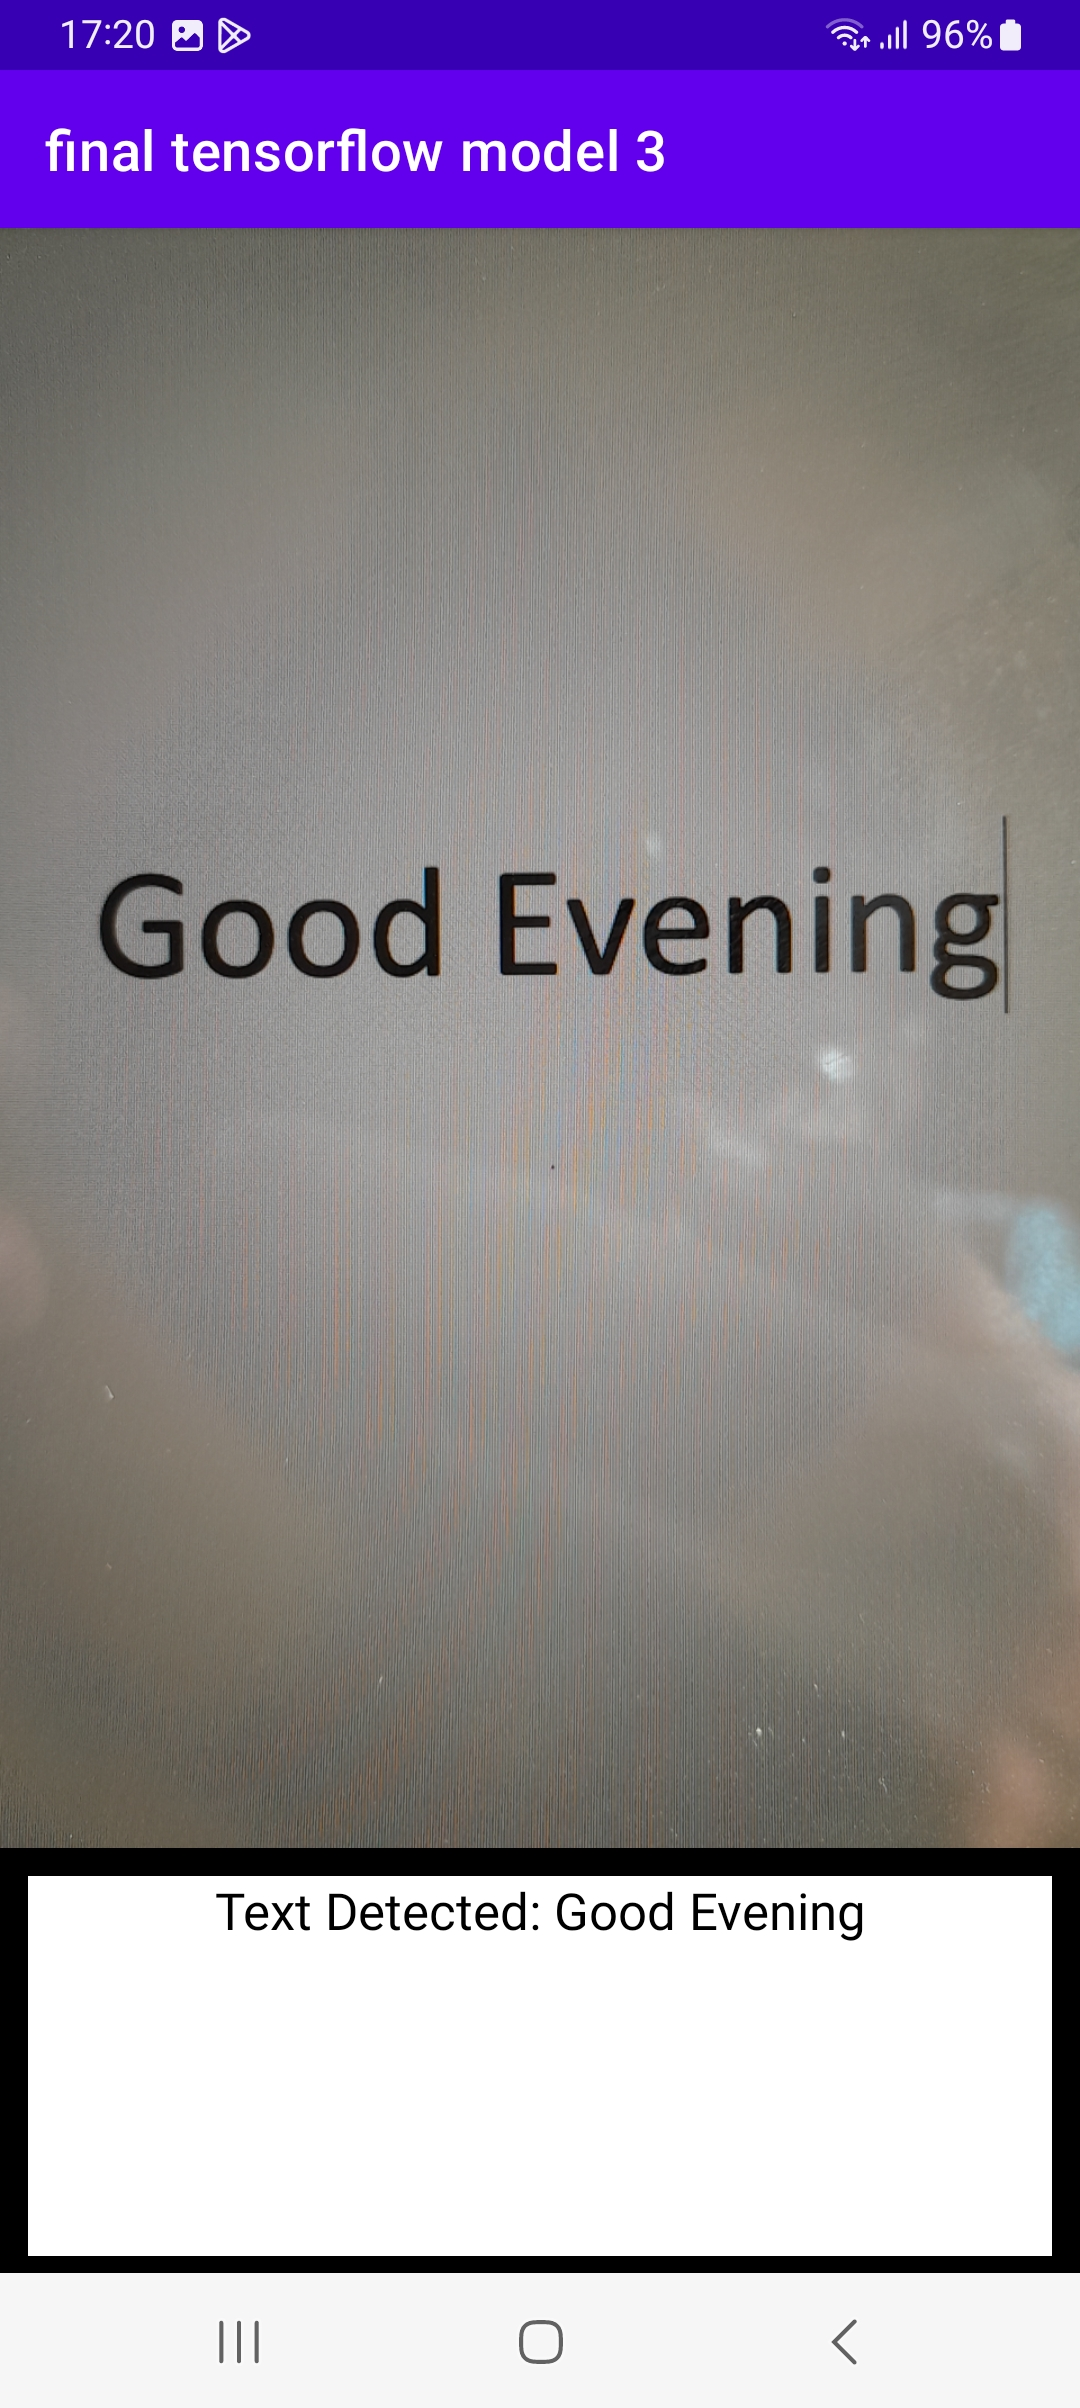
\includegraphics[width=0.23\linewidth]{Figures/Textwithwhite.jpg}}\hfill
    \subcaptionbox{\centering Text Captured in a Coloured Background}{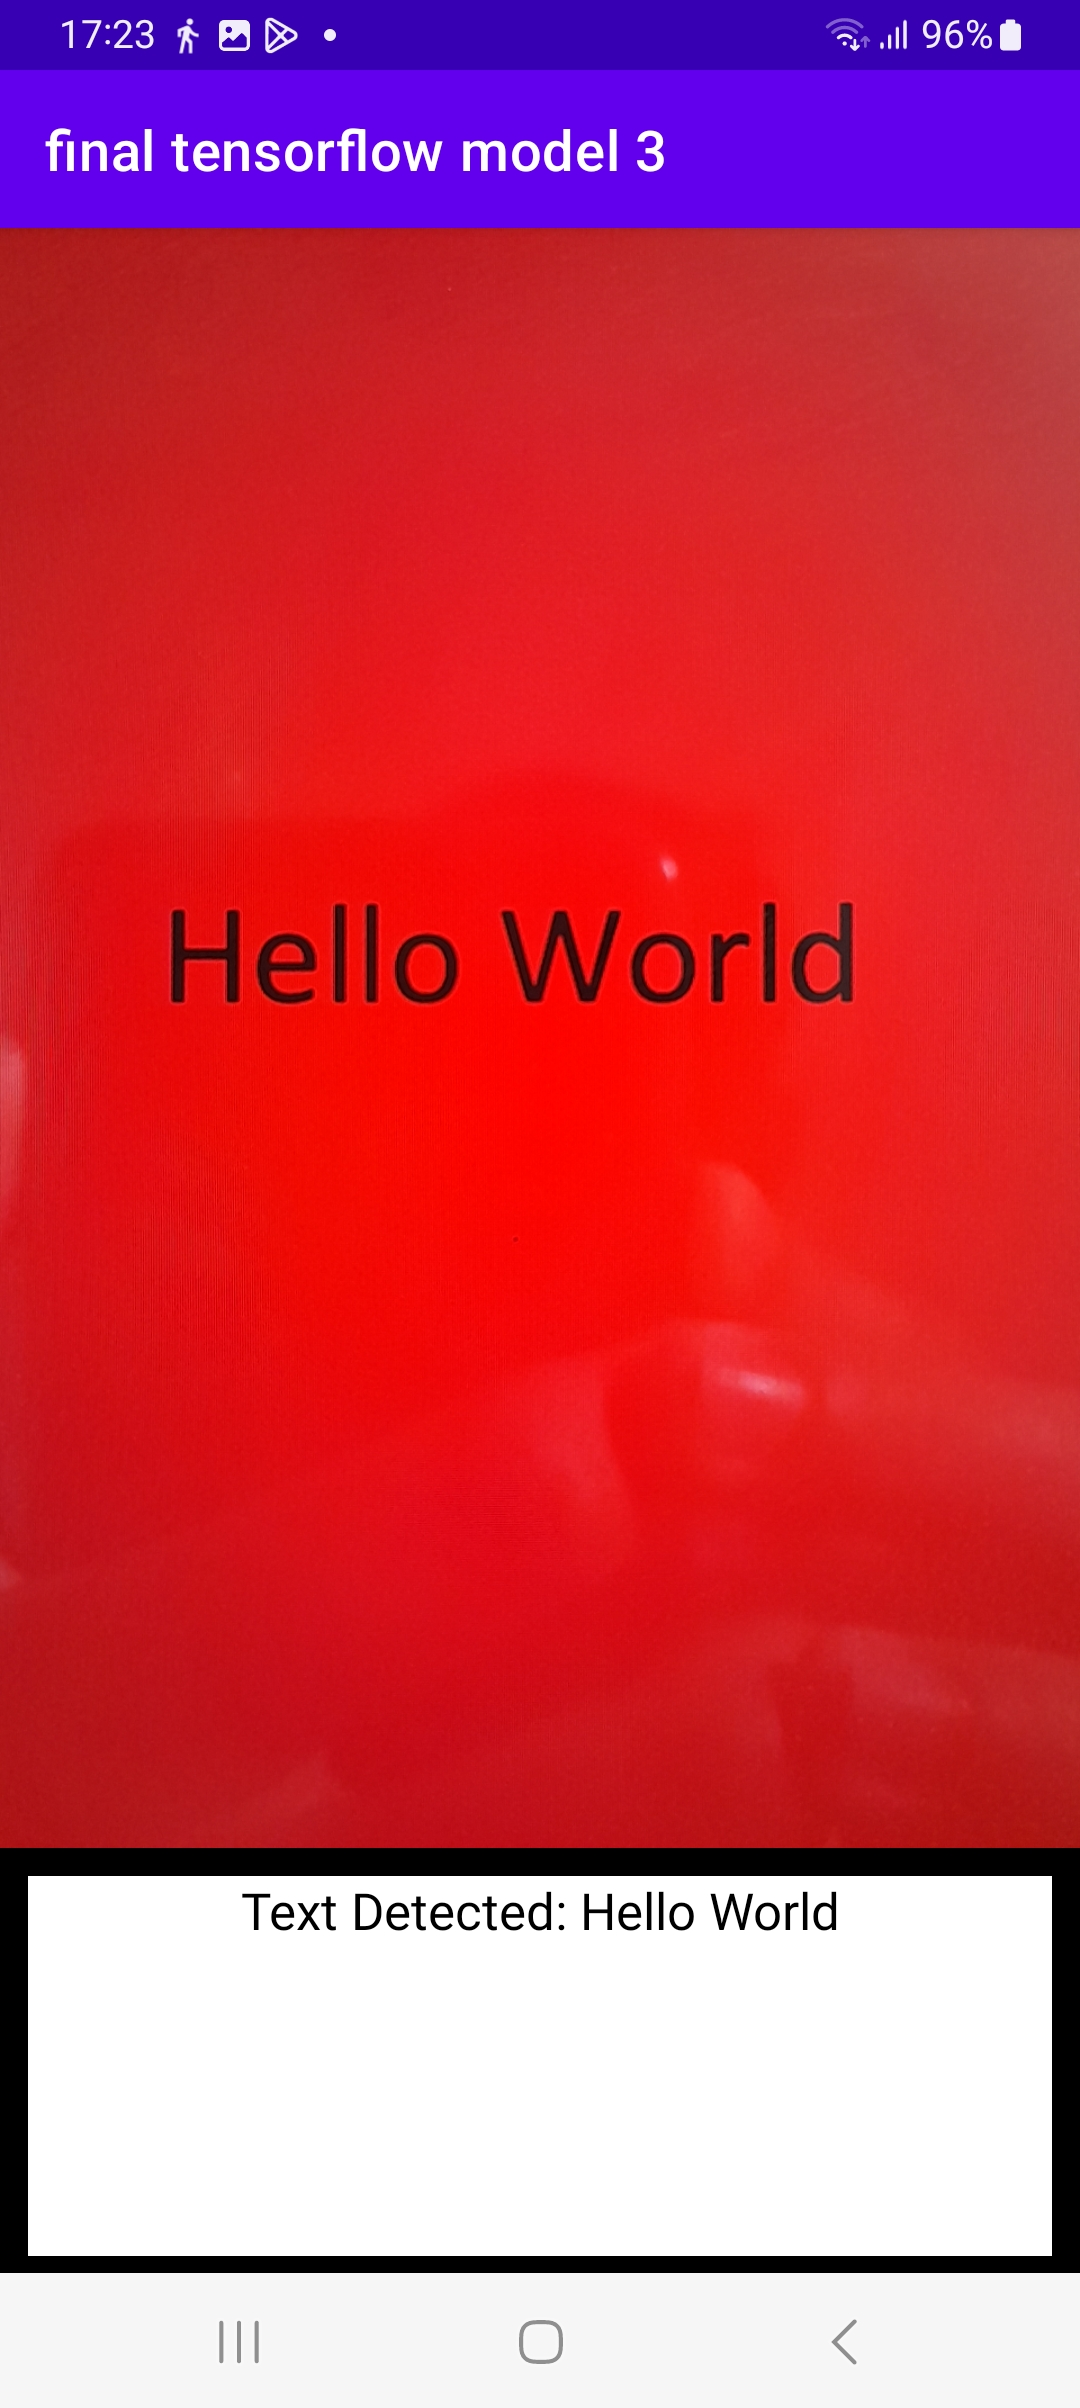
\includegraphics[width=0.23\linewidth]{Figures/Textwithcoloured.jpg}}\hfill
    \subcaptionbox{\centering Stop Sign Text Recognition}{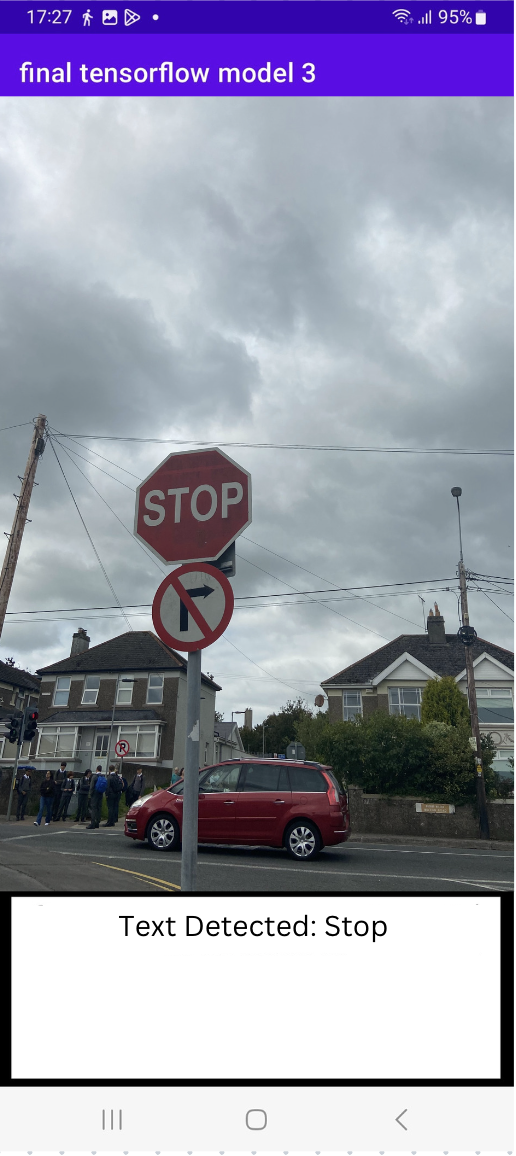
\includegraphics[width=0.23\linewidth]{Figures/Roadsign.png}}\hfill
    \subcaptionbox{ \centering Long Distance Text Recognition}{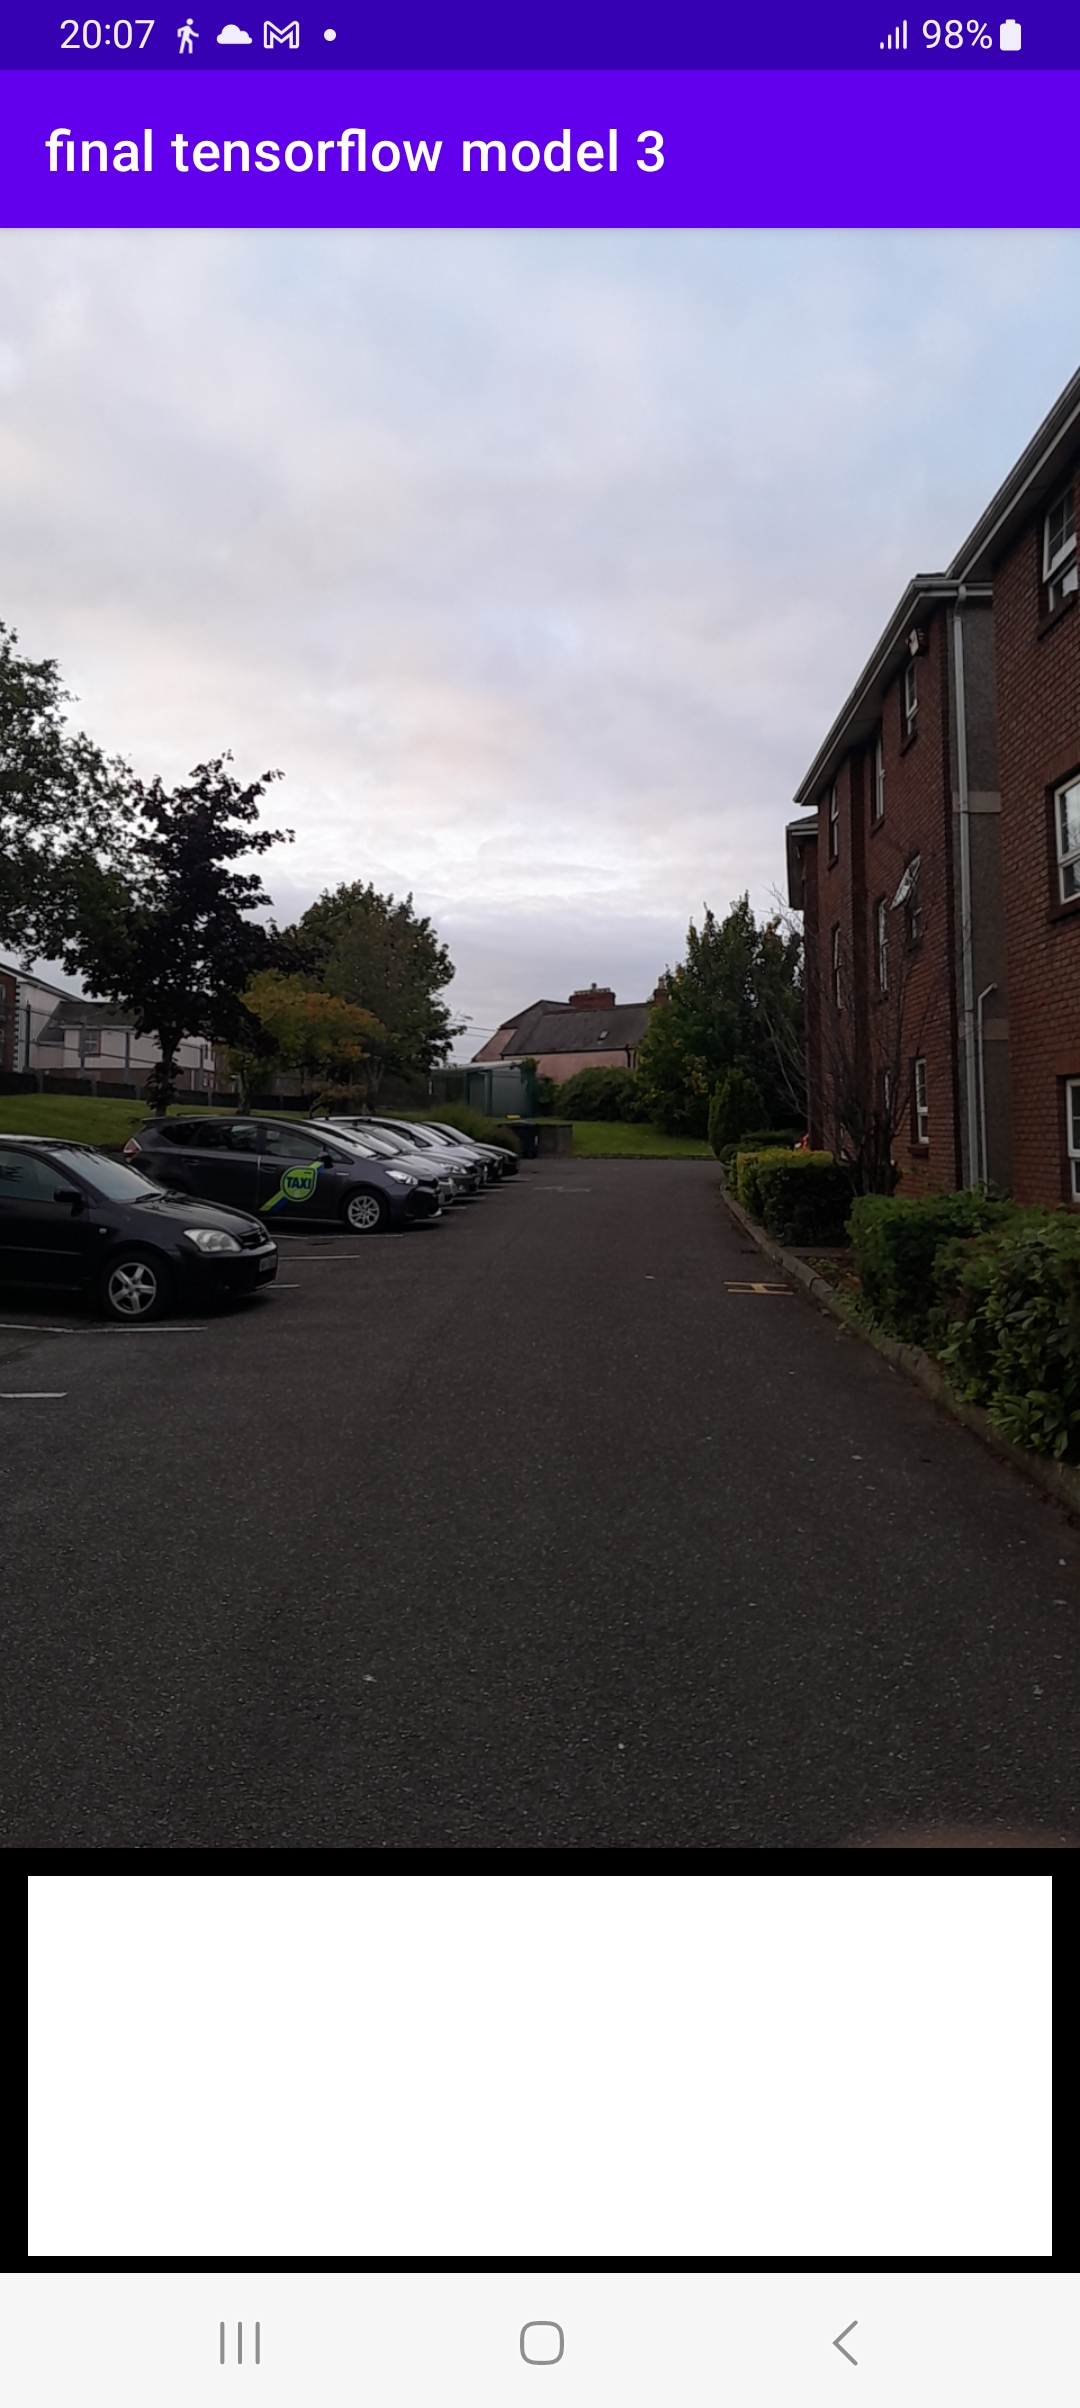
\includegraphics[width=0.23\linewidth]{Figures/TRFailed.jpg}}
    \caption{Output Images of the Functional Testing of Text Recognition}
\end{figure}


\end{enumerate}

\subsubsection{Feature 2: Object Recognition and Distance Evaluation}
\begin{enumerate}
    \item Test Case 1: Object placed at a Certain Distance
    \\The following test shows the application's behaviour when the Android device is placed in front of the chair as a object. The Output should display "Chair" and the distance of the chair.
    
    Result: PASS
     \item Test Case 2: Object placed in a low light room
    \\This test represents the application's response to the objects placed in a room with low light. The application should correctly detect all the objects in the picture. 
   
    Result: FAIL
    \item Test Case 3: Person with a Mobile Device
    \\Person using a mobile device has been given as a sample input for this test. The function should detect the person as well as mobile device in his hand.
   
    Result: PASS

    \item Test Case 4: Object Recognition and Distance Measurement in Low Light Area
    \\This test represents the application's response to the objects present in a low light area. The input image consist of three car which are more than 5 meters away. The application should correctly detect all the objects and provide the correct distance of it. 

   Result: FAIL

   \item Test Case 5: Object Recognition in Bright Light
    \\Object recognizer should provide all the objects in the image. The image contains objects like laptop and a cup

   Result: PASS

   \item Test Case 5: Traffic Lights
    This test shows the detection of the traffic light on the road. Th sample input is the image of the traffic light.

   Result: PASS

   \end{enumerate}

   \begin{figure}[H]
    \centering
    \subcaptionbox{\centering Chair at a Certain Distance}{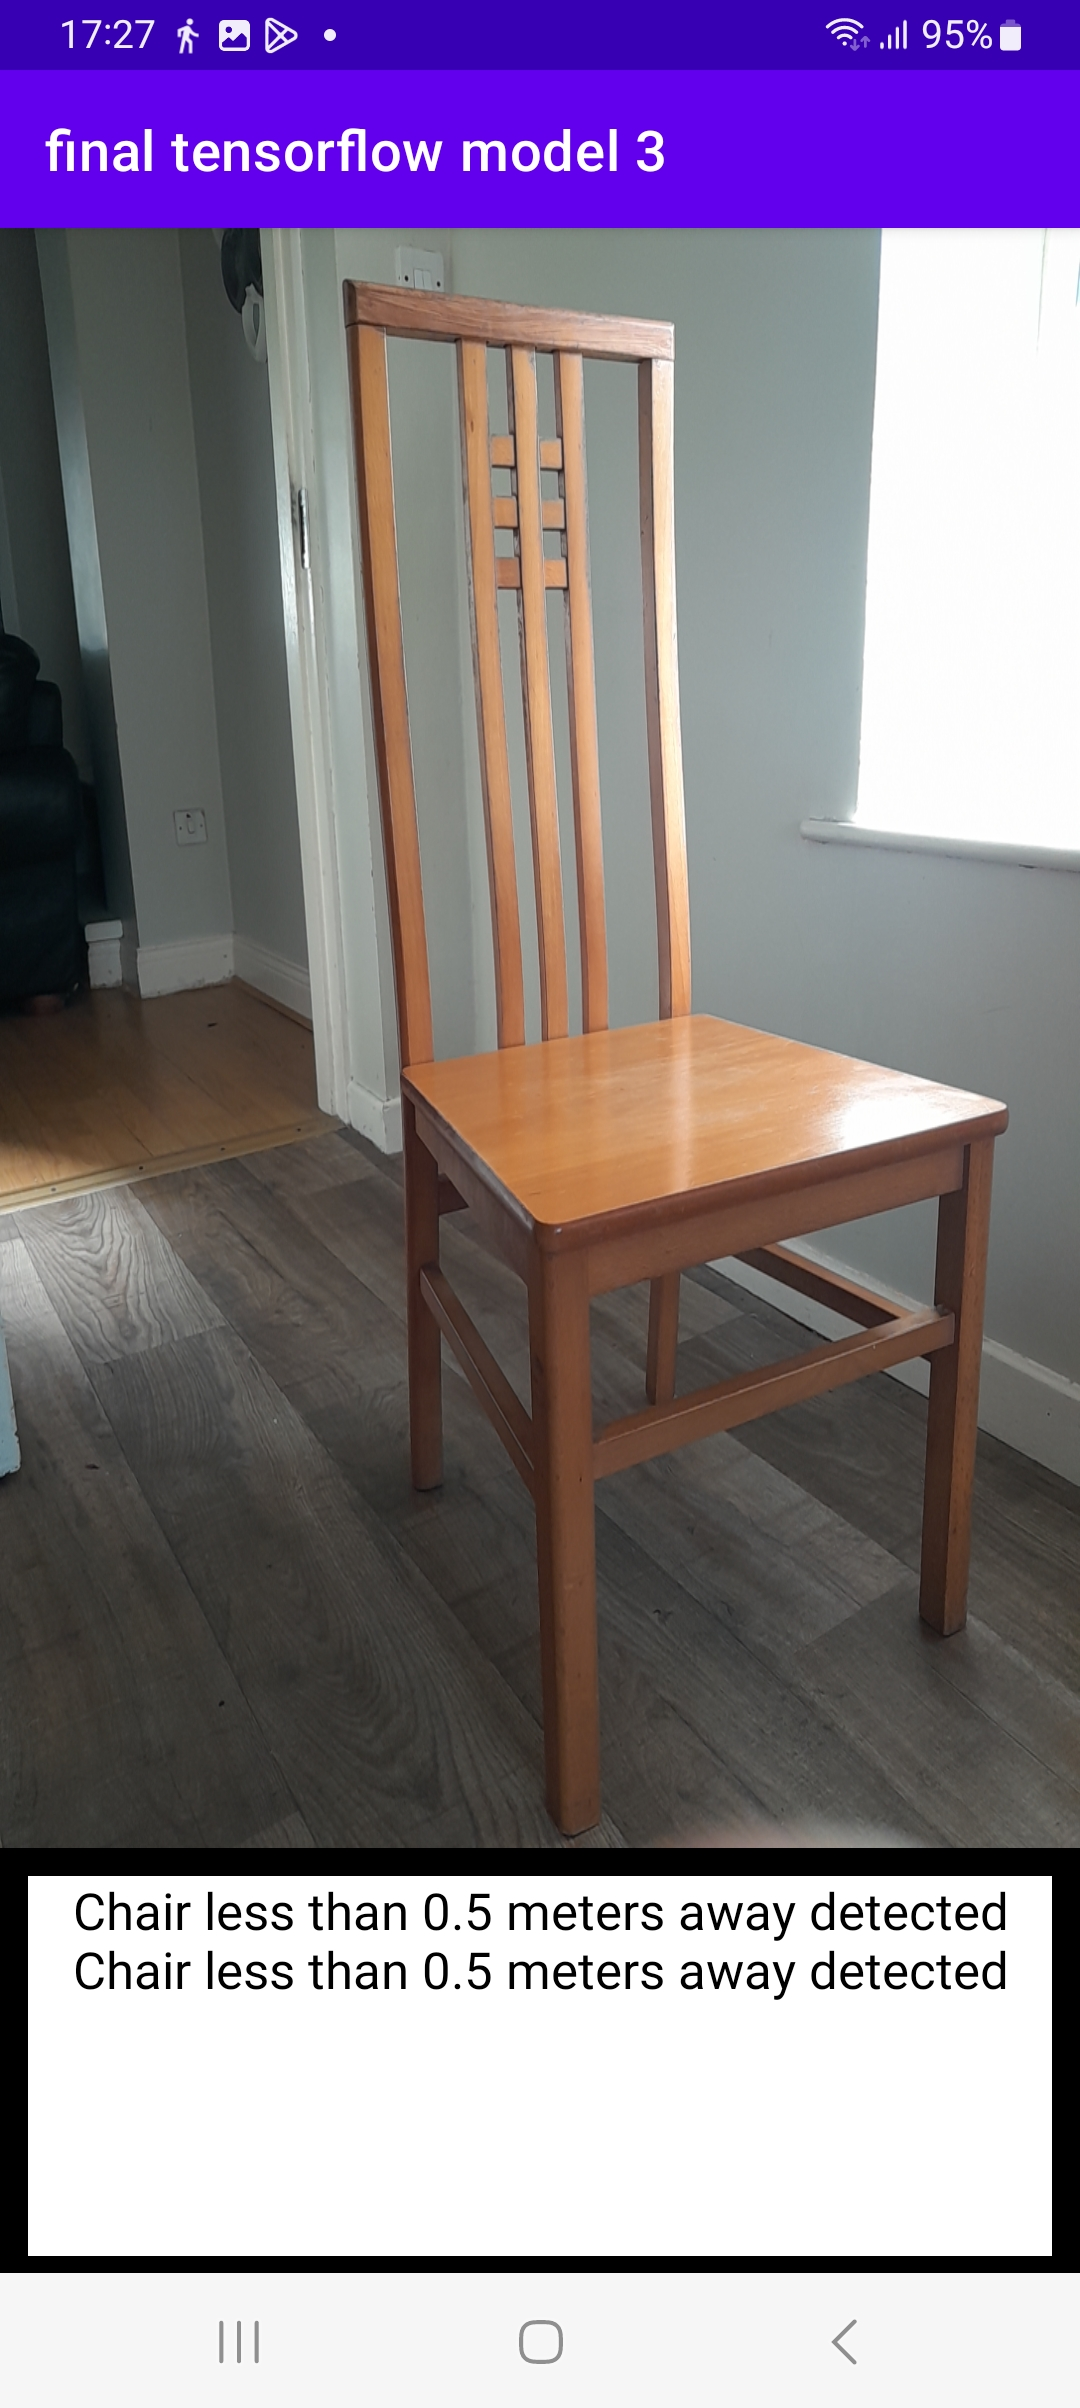
\includegraphics[width=0.27\linewidth]{Figures/Chair.jpg}}\hfill
    \subcaptionbox{\centering Objects placed in a Low Light Room}{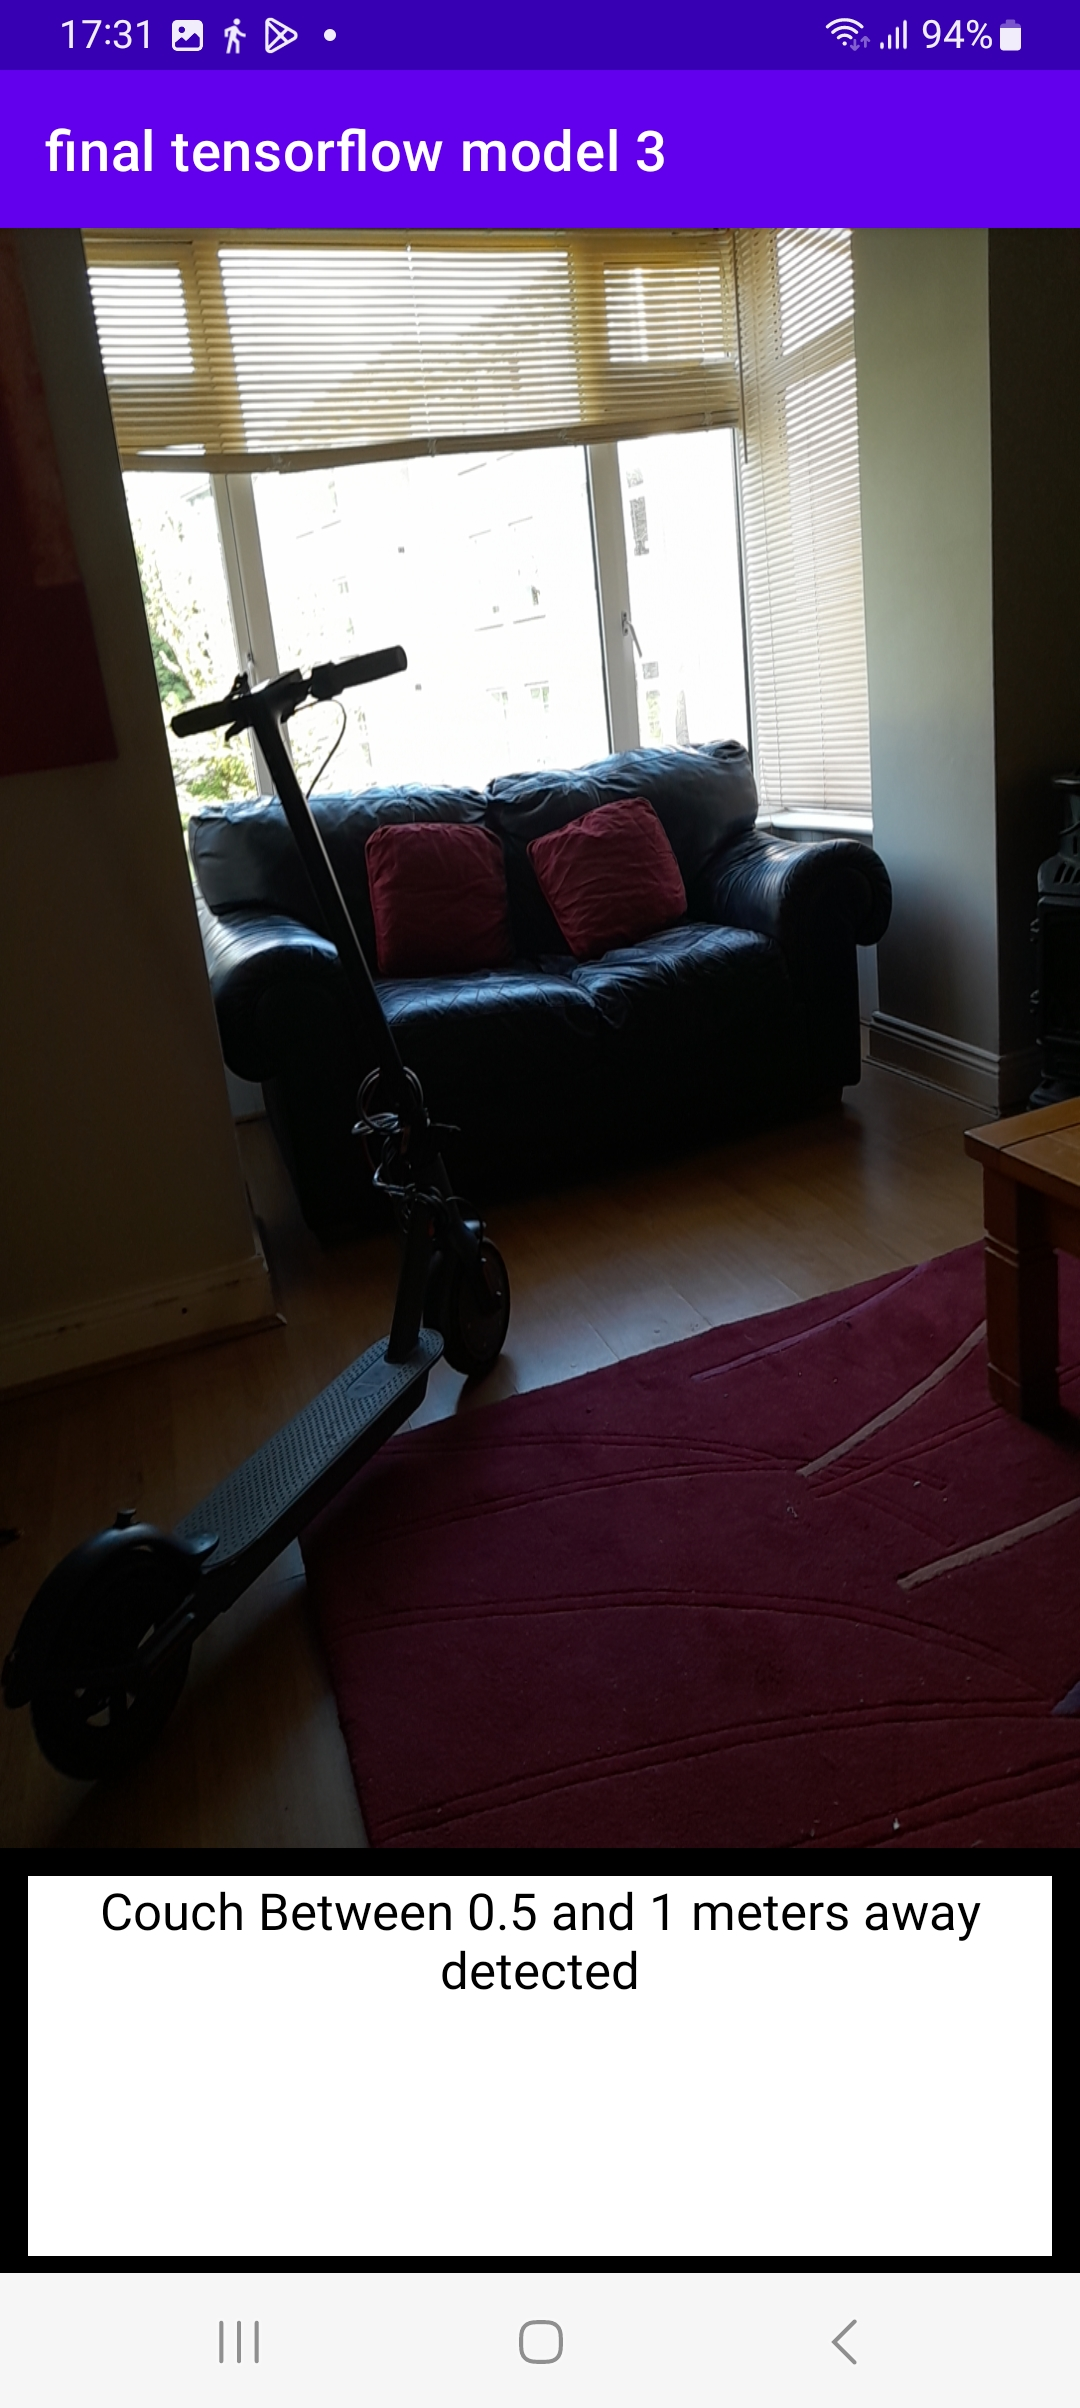
\includegraphics[width=0.27\linewidth]{Figures/Cycle_failed.jpg}}\hfill
    \subcaptionbox{\centering Person with a Mobile Device}{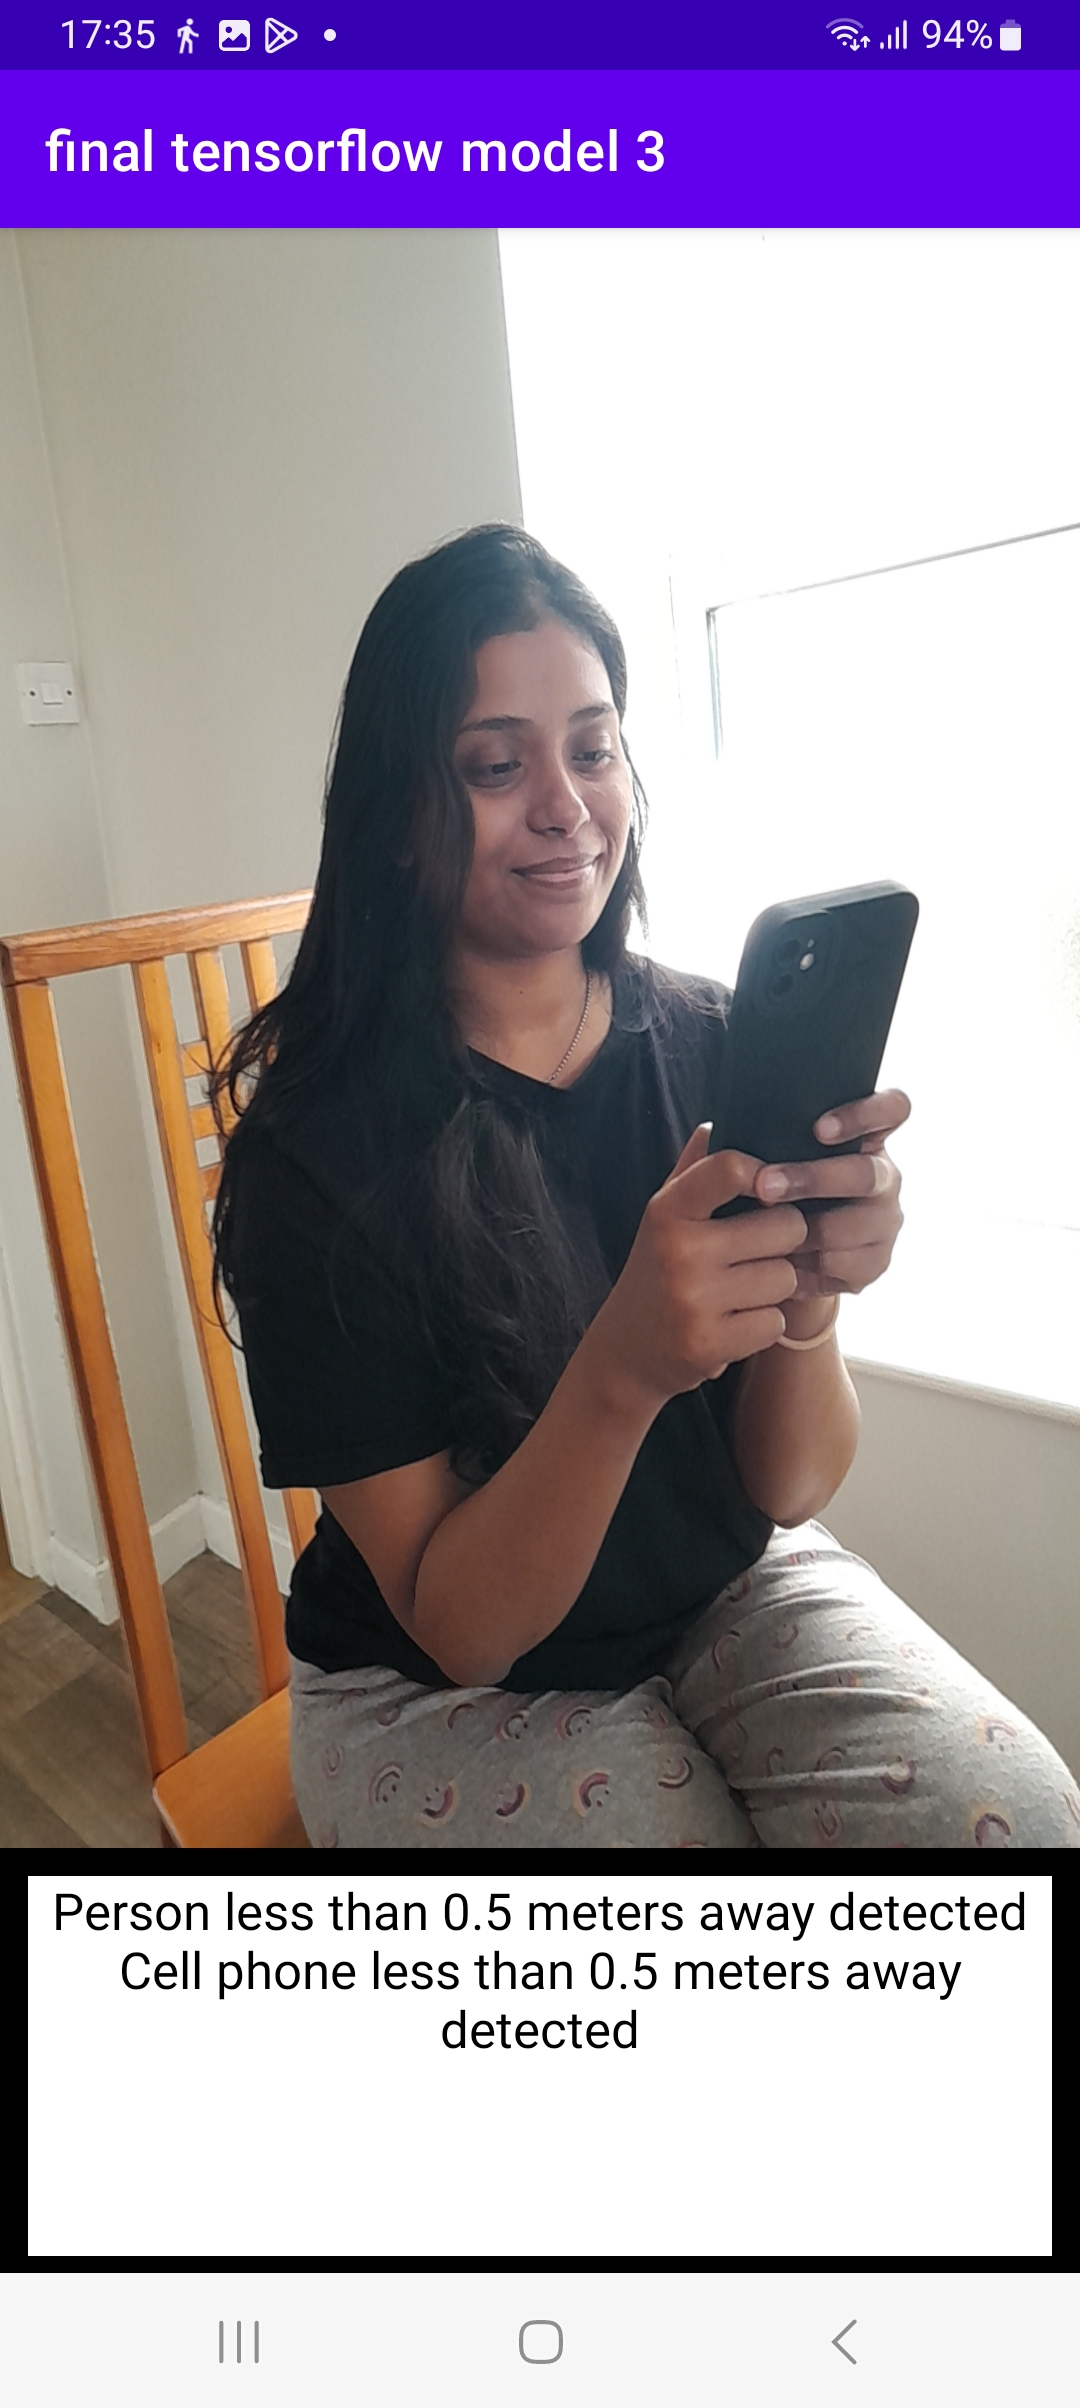
\includegraphics[width=0.27\linewidth]{Figures/Person.jpg}}\hfill
    \subcaptionbox{ \centering Cars in a Low Light Area }{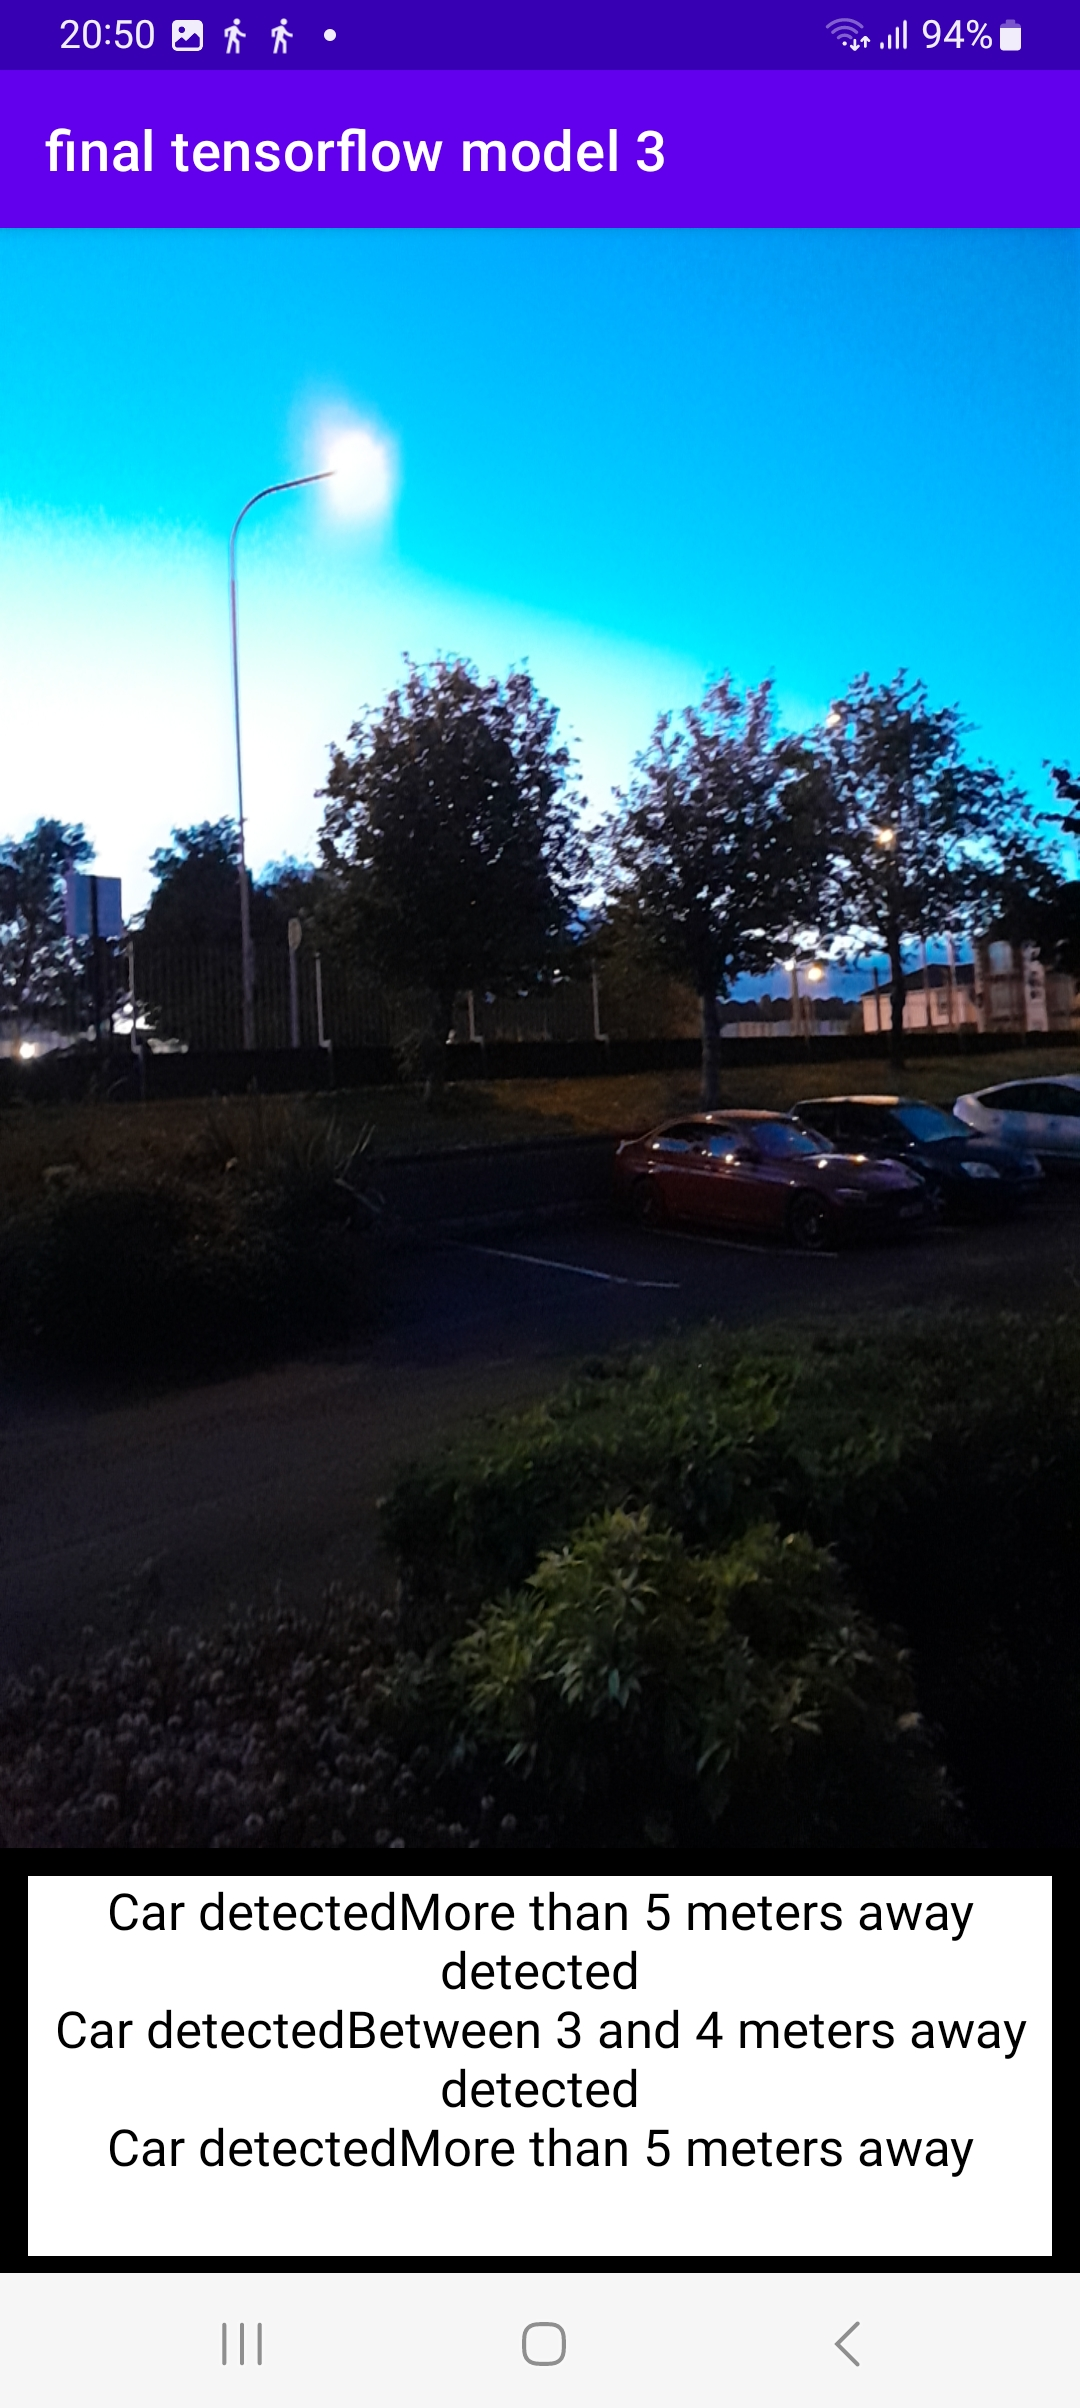
\includegraphics[width=0.27\linewidth]{Figures/car.jpg}}\hfill
    \subcaptionbox{ \centering Objects in a Bright Room }{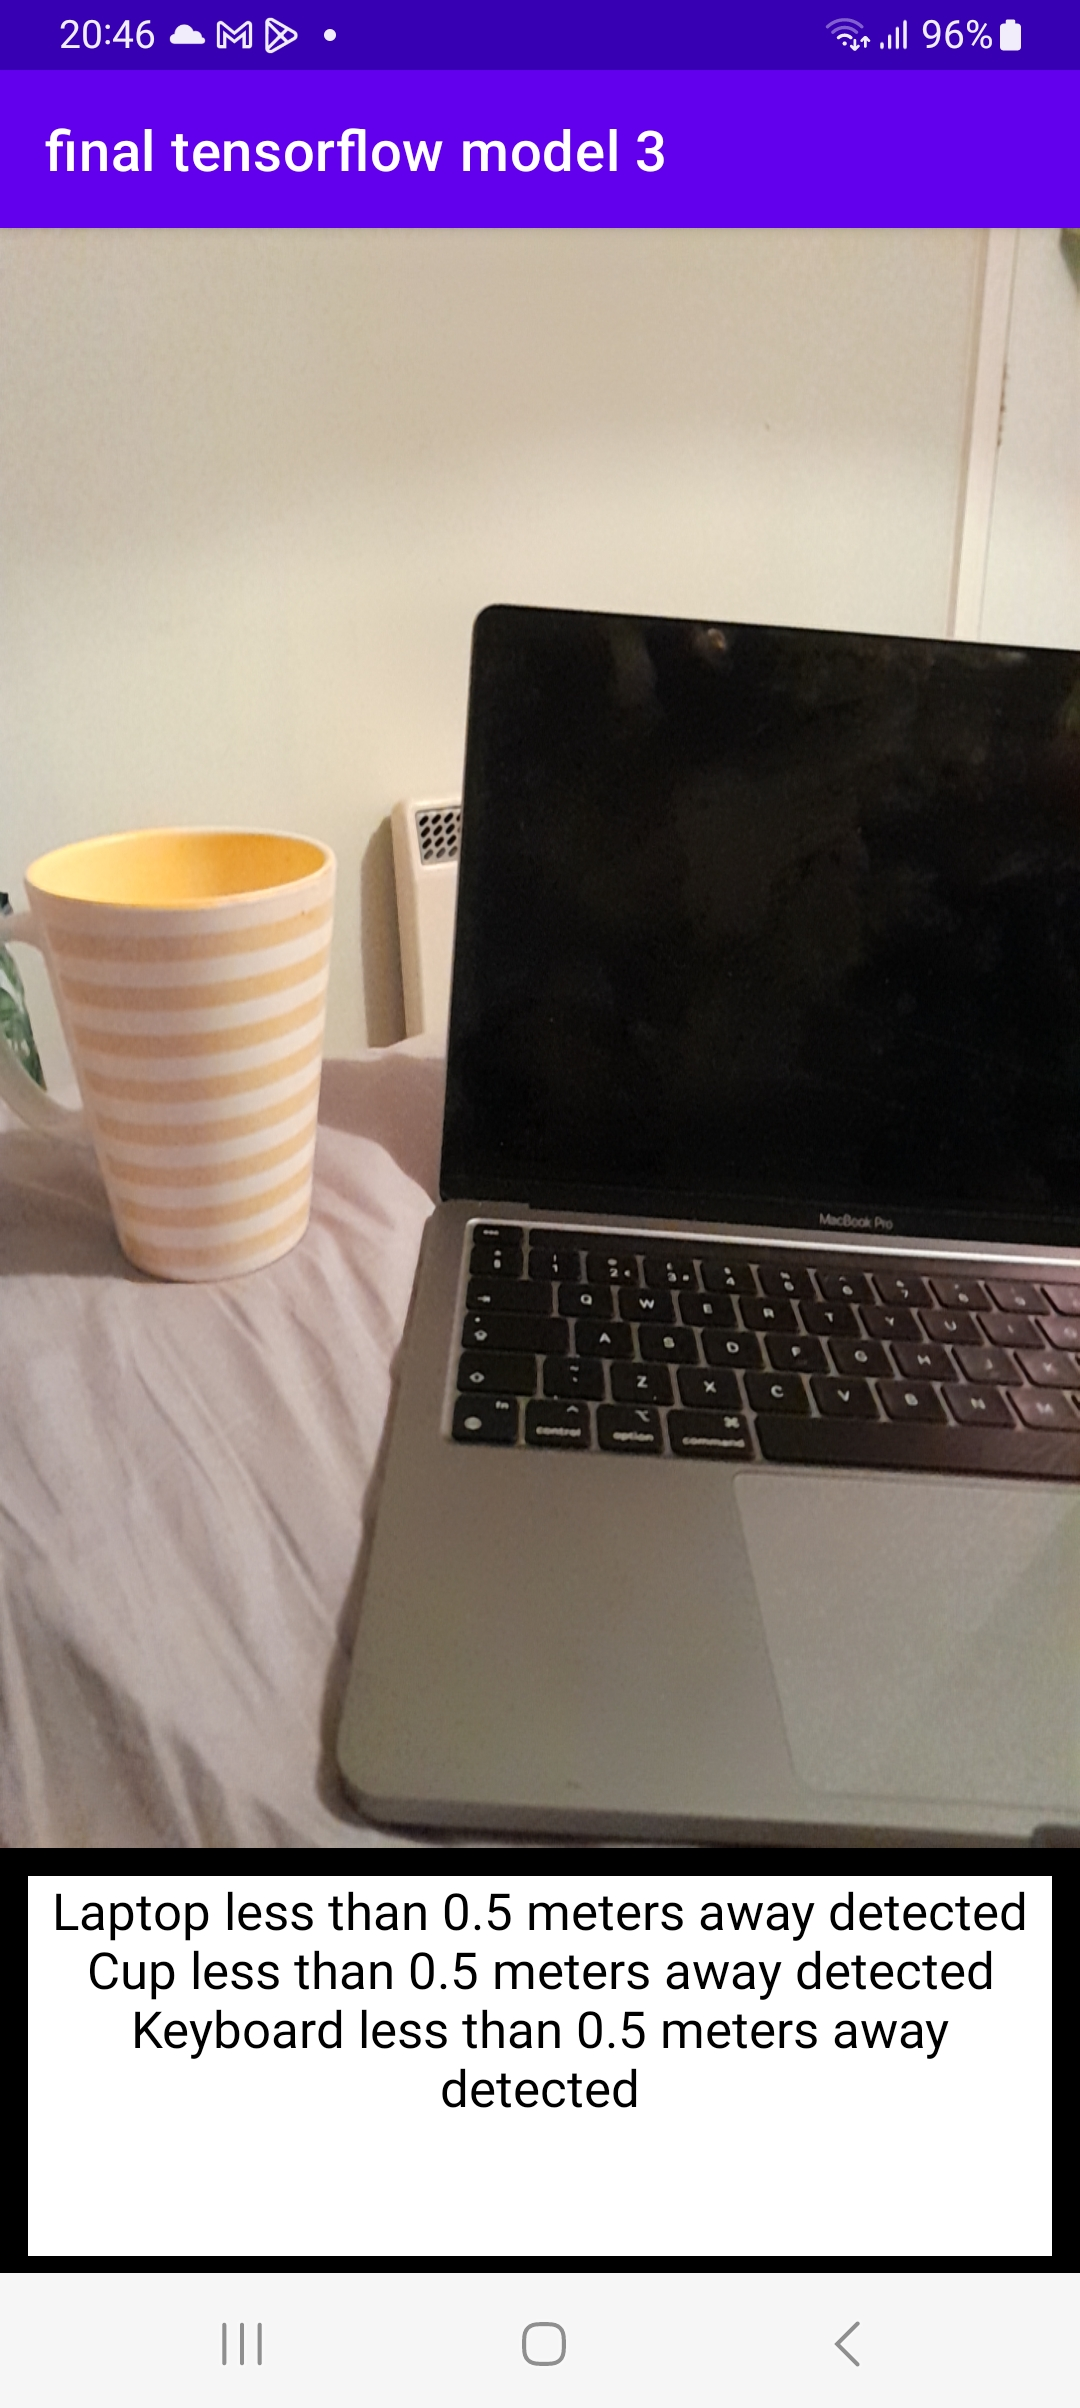
\includegraphics[width=0.27\linewidth]{Figures/LC.jpg}}\hfill
    \subcaptionbox{ \centering Traffic Lights }{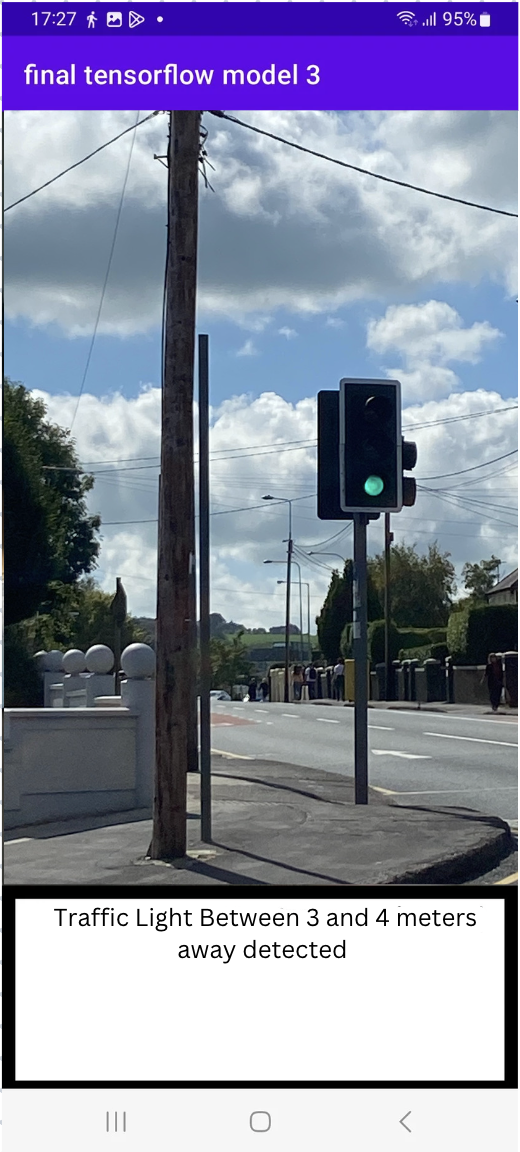
\includegraphics[width=0.27\linewidth]{Figures/TrafficLight.png}}
    \caption{Output Images of the Functional Testing of Object Recognition}
\end{figure}
\newpage\textbf{\\Approximate Output Values of Distance Calculation for all the Objects:-}
   
\begin{table}
  \centering
  \begin{tabular}{|c|c|}
    \hline
    \textbf{Objects} & \textbf{Distance (in Meters)}  \\
    \hline
    Chair & 0.312455  \\
    \hline
    Couch & 0.915223  \\
    \hline
    Person & 0.456179  \\
    \hline
    Mobile & 0.251678  \\
    \hline
    Car 1 & 7.891459  \\
    \hline
    Car 2 & 3.789103  \\
    \hline
    Car 3 & 8.984680  \\
    \hline
    Laptop & 0.103489  \\
    \hline
    Cup & 0.122068  \\
    \hline
    Keyboard & 0.098729  \\
    \hline
    Traffic Lights & 3.980568  \\
    \hline
  \end{tabular}
  \caption{Precise measurements obtained during distance estimation}
\end{table}

\subsubsection{Feature 3: Audio Feedback}
\begin{enumerate}
    \item Test Case 1: Audio response when Text is detected
    \\This test presents Audio response when the text is detected by the application. The Audio should provide clear information about the text detected 
    \\Result: PASS
     \item Test Case 2: Audio response when Object is detected
    \\Audio feedback when the object is detected by the application has been recorded in this test.
    \\Result: PASS
   
\end{enumerate}

\subsection{Test Environment}

The environment for the test has been setup so the it could depict the real-world environment as closely as possible. Various light conditions, coloured backgrounds and different font sizes for the text recognition tests has been included in the environment. Also the real time information provided by the application has been checked to help the visually impaired individuals.

\subsection{Test Results}
\begin{itemize}
    \item Overall Test Cases Executed- A total of 9 Test cases has been tested while functional testing of the application.
    \item Cases Passed- 7 of the run scenarios succeeded without any difficulties. These examples comprised instances in which the program accurately detected and supported visually challenged users.
    \item Cases Failed- 2 test scenarios did not yield the intended results. Inconsistencies were classified as either crucial or non-essential tasks depending on their influence on the application's fundamental functions.
\end{itemize}


\subsection{Functional Testing Conclusion}

The efficiency, dependability, and accessibility of the program for those with vision impairment assistance have been much improved as a result of the practical evaluation phase. The tool performed well in identifying and recognizing information from a variety of everyday situations. The content size, style, and layout instances in the test regularly generated good results. Also for the Object Recognition and Distance Evaluation every aspect of the scenario has been tested. The program continuously gave precise information about items and how far they were from the user, greatly enhancing user safety.


\section{Usability Testing}
\subsection{Introduction}

Usability Testing phase has been detailed in this section providing the feedback of the users and the it also explains how well the application meets the needs of the target users.
\\Objectives of this test are as follows:
\begin{enumerate}
    \item To evaluate the performance, usability and user-friendliness of the application.
    \item To research all the areas of improvements encountered during the use.
    \item To gain users feedback and make necessary improvements.
\end{enumerate}

\subsection{Methodology}
\subsubsection{Participants}
All the participants in these testing have been chosen very carefully so they can reflect the intended users consisting visual impaired individuals. The testing method involved an overall of 4 people. The Age range of the participants varied from 25 years - 40 years. 3 of the participants involved in the testing had low vision eyesight and the one was blind. 

\subsubsection{Testing Environment}
To guarantee the ease and security of the subjects, evaluation of usability test was carried out in a regulated and friendly setting. The location of the park was chosen for the experiment because of its easy access and tranquil environs. The participants were encouraged to use there own Android Smartphones as this will depict the real world scenario for them.

\subsubsection{Tasks}

This test involved a series of task which mimics the real-world situations for visual impaired individuals. The exercises were designed specifically for the people who are blind. The tasks consisted of:-

\begin{enumerate}
    \item Task 1:- 
    \\ Open the application and roam around the locality.
    \item Task 2:-
    \\Switch to Text Mode and let the app read aloud the sign board on the road.
    \item Task 3:-
    \\Interact with the application, let the application detect various objects and their distances.
    \item Task 4:-
    \\Toggle through the application's different modes of operation.
\end{enumerate}

\subsubsection{Process}
The testing  was done by following a defined procedure so it can ensure uniformity and make information collection easier. The participants were briefly instructed through the overall process and each of the subject gave their informed permission. They were given particular accomplishments to achieve. Throughout the test period, they were urged to speak out loud and offer their ideas. Participants were provided with the overview of the application. Observations were taken into account while the participants were doing their given tasks. After the procedure was completed and the participants did all the tasks given to them, they were given the chance to give a general feedback on the overall experience. Data was collected from all the users and the detailed observations were made noting all the difficulties faced by the user.

\subsection{Results}
In this section we represent all the quantitative data, qualitative data and usability issues faced by the individuals.
These measurements give a statistical view on how well the application is used by the participants.
 \begin{figure}[H]
      \hrule
      \vspace{0.5em}
     \centering
      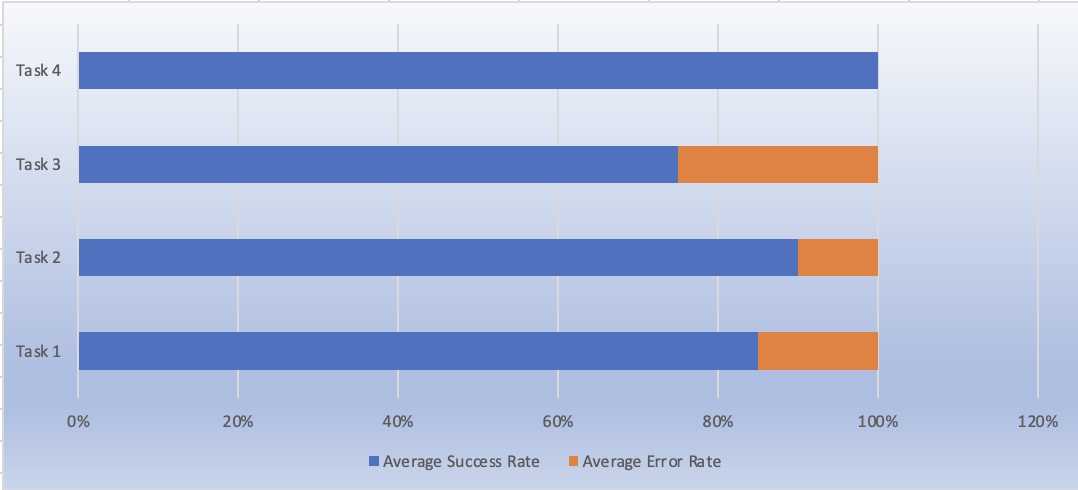
\includegraphics[width=0.9\textwidth]{Figures/SRVSER.png}
      \vspace{0.5em}
      \hrule
      \caption{\centering\label{fig:SRVSER}Rates for Completion of Tasks}
      \vspace{0.5em}
      \hrule
   \end{figure}

   The above Figure \ref{fig:SRVSER} shows the success rate of the task with respect to the error rates encountered by the participants. All the task were examined and performed in a given time frame of 10 minutes. The task which has the lowest success rate was "Task 3" which was to let the application detect all the objects in the surrounding. The application could not detect some of the objects in the environment and the application recognized some of the objects as "Unknown Objects". 

   The Participants also gave a valuable feedback on the application such as:-
   \begin{enumerate}
       \item Participant 1:- "The application detected a lot of objects in the way and the distance estimation is a good feature to add."
       \item Participant 2:- "Text Detection can be Improved."
       \item Participant 3:- "Audio Feedback approach is a nice way to give visual Impaired Individual information about the surrounding."
       \item Participant 4:- "Distance Estimation can be more accurate."
   \end{enumerate}

\subsubsection{Usability Testing Conclusion}

The results of the usability evaluation performed for the application have been thoroughly reviewed in this chapter. The system undergone a thorough examination to determine its efficacy, convenience, and user interface. It was painstakingly created in response to the special needs of those who are visually impaired. The feedback of the participants have been taken into consideration. Future development and enhancement of an application will be built around the findings of the usability evaluation as a strong basis. 


\chapter{Conclusion}

Through the creation of a complete mobile application, we set out on a mission to improve the level of daily life of people who are blind or visually impaired. The difficulties which those with vision impairments encounter on every day, such as recognising text, object identification, and distance measurement, served as the inspiration for this project. The objective we set was to develop a device that will enable people to conquer these barriers, reclaim their freedom, and confidently travel across the globe without fear.

\section{Key Achievements}

The Application has conquered various challenges which were encountered by the visual impaired individuals all the time while roaming out of the house. The applications can do a lot of work including determining objects and measuring the distance to the object, identifying a person and recognition of text which will help the users to read any road signs or directions on their way. It can also seamlessly switch between two activities without any interruptions with a audio feedback when the user switches the screen. This approach also provides audio output of the objects or texts it detects making the life easier for visually impaired individuals.

\section{Future Work}

The app we developed may act as a base for potential enhancements as science develops and customer requests change. The Future Work includes development of the navigational features which can provide accurate directions to the users throughout their outdoor journey. The design of the application displays a simple and easy to use interface. The features and functionality of the app will need to be improved and expanded by cooperation with other groups of people who are visually impaired and subject matter specialists. Also implementing a auto zoom feature for the text recognition system is also considered as a future implementation in this application as this will auto zoom the camera to the text in the vicinity of the user and can let him know about that text prior.

\section{Summary}

As a result of our thesis research, an application that will assist people who are blind in everyday tasks has been developed. In addition to producing a useful instrument, the creation approach served as a reminder of the value of approachable innovations for solving practical problems.
\\We are dedicated to ongoing growth and creativity while we move to the years to come, influenced by the values of transparency and inclusion. We want to contribute to making the global community open and egalitarian for everyone via constant cooperation, evaluation, and improvement.





\
%
%
\backmatter
%
%
   \printbibliography
\end{document}
